% Options for packages loaded elsewhere
\PassOptionsToPackage{unicode}{hyperref}
\PassOptionsToPackage{hyphens}{url}
%
\documentclass[
]{article}
\usepackage{amsmath,amssymb}
\usepackage{iftex}
\ifPDFTeX
  \usepackage[T1]{fontenc}
  \usepackage[utf8]{inputenc}
  \usepackage{textcomp} % provide euro and other symbols
\else % if luatex or xetex
  \usepackage{unicode-math} % this also loads fontspec
  \defaultfontfeatures{Scale=MatchLowercase}
  \defaultfontfeatures[\rmfamily]{Ligatures=TeX,Scale=1}
\fi
\usepackage{lmodern}
\ifPDFTeX\else
  % xetex/luatex font selection
\fi
% Use upquote if available, for straight quotes in verbatim environments
\IfFileExists{upquote.sty}{\usepackage{upquote}}{}
\IfFileExists{microtype.sty}{% use microtype if available
  \usepackage[]{microtype}
  \UseMicrotypeSet[protrusion]{basicmath} % disable protrusion for tt fonts
}{}
\makeatletter
\@ifundefined{KOMAClassName}{% if non-KOMA class
  \IfFileExists{parskip.sty}{%
    \usepackage{parskip}
  }{% else
    \setlength{\parindent}{0pt}
    \setlength{\parskip}{6pt plus 2pt minus 1pt}}
}{% if KOMA class
  \KOMAoptions{parskip=half}}
\makeatother
\usepackage{xcolor}
\usepackage[margin=1in]{geometry}
\usepackage{color}
\usepackage{fancyvrb}
\newcommand{\VerbBar}{|}
\newcommand{\VERB}{\Verb[commandchars=\\\{\}]}
\DefineVerbatimEnvironment{Highlighting}{Verbatim}{commandchars=\\\{\}}
% Add ',fontsize=\small' for more characters per line
\usepackage{framed}
\definecolor{shadecolor}{RGB}{248,248,248}
\newenvironment{Shaded}{\begin{snugshade}}{\end{snugshade}}
\newcommand{\AlertTok}[1]{\textcolor[rgb]{0.94,0.16,0.16}{#1}}
\newcommand{\AnnotationTok}[1]{\textcolor[rgb]{0.56,0.35,0.01}{\textbf{\textit{#1}}}}
\newcommand{\AttributeTok}[1]{\textcolor[rgb]{0.13,0.29,0.53}{#1}}
\newcommand{\BaseNTok}[1]{\textcolor[rgb]{0.00,0.00,0.81}{#1}}
\newcommand{\BuiltInTok}[1]{#1}
\newcommand{\CharTok}[1]{\textcolor[rgb]{0.31,0.60,0.02}{#1}}
\newcommand{\CommentTok}[1]{\textcolor[rgb]{0.56,0.35,0.01}{\textit{#1}}}
\newcommand{\CommentVarTok}[1]{\textcolor[rgb]{0.56,0.35,0.01}{\textbf{\textit{#1}}}}
\newcommand{\ConstantTok}[1]{\textcolor[rgb]{0.56,0.35,0.01}{#1}}
\newcommand{\ControlFlowTok}[1]{\textcolor[rgb]{0.13,0.29,0.53}{\textbf{#1}}}
\newcommand{\DataTypeTok}[1]{\textcolor[rgb]{0.13,0.29,0.53}{#1}}
\newcommand{\DecValTok}[1]{\textcolor[rgb]{0.00,0.00,0.81}{#1}}
\newcommand{\DocumentationTok}[1]{\textcolor[rgb]{0.56,0.35,0.01}{\textbf{\textit{#1}}}}
\newcommand{\ErrorTok}[1]{\textcolor[rgb]{0.64,0.00,0.00}{\textbf{#1}}}
\newcommand{\ExtensionTok}[1]{#1}
\newcommand{\FloatTok}[1]{\textcolor[rgb]{0.00,0.00,0.81}{#1}}
\newcommand{\FunctionTok}[1]{\textcolor[rgb]{0.13,0.29,0.53}{\textbf{#1}}}
\newcommand{\ImportTok}[1]{#1}
\newcommand{\InformationTok}[1]{\textcolor[rgb]{0.56,0.35,0.01}{\textbf{\textit{#1}}}}
\newcommand{\KeywordTok}[1]{\textcolor[rgb]{0.13,0.29,0.53}{\textbf{#1}}}
\newcommand{\NormalTok}[1]{#1}
\newcommand{\OperatorTok}[1]{\textcolor[rgb]{0.81,0.36,0.00}{\textbf{#1}}}
\newcommand{\OtherTok}[1]{\textcolor[rgb]{0.56,0.35,0.01}{#1}}
\newcommand{\PreprocessorTok}[1]{\textcolor[rgb]{0.56,0.35,0.01}{\textit{#1}}}
\newcommand{\RegionMarkerTok}[1]{#1}
\newcommand{\SpecialCharTok}[1]{\textcolor[rgb]{0.81,0.36,0.00}{\textbf{#1}}}
\newcommand{\SpecialStringTok}[1]{\textcolor[rgb]{0.31,0.60,0.02}{#1}}
\newcommand{\StringTok}[1]{\textcolor[rgb]{0.31,0.60,0.02}{#1}}
\newcommand{\VariableTok}[1]{\textcolor[rgb]{0.00,0.00,0.00}{#1}}
\newcommand{\VerbatimStringTok}[1]{\textcolor[rgb]{0.31,0.60,0.02}{#1}}
\newcommand{\WarningTok}[1]{\textcolor[rgb]{0.56,0.35,0.01}{\textbf{\textit{#1}}}}
\usepackage{graphicx}
\makeatletter
\def\maxwidth{\ifdim\Gin@nat@width>\linewidth\linewidth\else\Gin@nat@width\fi}
\def\maxheight{\ifdim\Gin@nat@height>\textheight\textheight\else\Gin@nat@height\fi}
\makeatother
% Scale images if necessary, so that they will not overflow the page
% margins by default, and it is still possible to overwrite the defaults
% using explicit options in \includegraphics[width, height, ...]{}
\setkeys{Gin}{width=\maxwidth,height=\maxheight,keepaspectratio}
% Set default figure placement to htbp
\makeatletter
\def\fps@figure{htbp}
\makeatother
\setlength{\emergencystretch}{3em} % prevent overfull lines
\providecommand{\tightlist}{%
  \setlength{\itemsep}{0pt}\setlength{\parskip}{0pt}}
\setcounter{secnumdepth}{-\maxdimen} % remove section numbering
\ifLuaTeX
  \usepackage{selnolig}  % disable illegal ligatures
\fi
\IfFileExists{bookmark.sty}{\usepackage{bookmark}}{\usepackage{hyperref}}
\IfFileExists{xurl.sty}{\usepackage{xurl}}{} % add URL line breaks if available
\urlstyle{same}
\hypersetup{
  pdftitle={Structure and Function of the Soil Microbiome Underlying N2O Emissions from Global Wetlands},
  hidelinks,
  pdfcreator={LaTeX via pandoc}}

\title{Structure and Function of the Soil Microbiome Underlying N2O
Emissions from Global Wetlands}
\author{Mohammad Bahram1,2,9, Mikk Espenberg1,9, Jaan Pärn1,9, Laura
Lehtovirta-Morley3,\\
Sten Anslan1, Kuno Kasak1, Urmas Kõljalg1, Jaan Liira1, Martin
Maddison1,\\
Mari Moora1, Ülo Niinemets4, Maarja Öpik1, Meelis Pärtel1, Kaido
Soosaar1,\\
Martin Zobel1, Falk Hildebrand5,6, Leho Tedersoo7,8,9, Ülo Mander1,9}
\date{}

\begin{document}
\maketitle

{
\setcounter{tocdepth}{2}
\tableofcontents
}
\begin{enumerate}
\def\labelenumi{\arabic{enumi}.}
\tightlist
\item
  \textbf{Institute of Ecology and Earth Sciences}, University of Tartu,
  Tartu, Estonia.\\
\item
  \textbf{Department of Ecology}, Swedish University of Agricultural
  Sciences, Uppsala, Sweden.\\
\item
  \textbf{School of Biological Sciences}, University of East Anglia,
  Norwich, UK.\\
\item
  \textbf{Institute of Agricultural \& Environmental Sciences}, Estonian
  University of Life Sciences, Tartu, Estonia.\\
\item
  \textbf{Quadram Institute Bioscience}, Norwich, Norfolk, UK.\\
\item
  \textbf{Digital Biology}, Earlham Institute, Norwich, Norfolk, UK.\\
\item
  \textbf{College of Science}, King Saud University, Riyadh, Saudi
  Arabia.\\
\item
  \textbf{Mycology and Microbiology Center}, University of Tartu, Tartu,
  Estonia.\\
\item
  \textbf{These authors contributed equally}: Mohammad Bahram, Mikk
  Espenberg, Jaan Pärn, Leho Tedersoo, Ülo Mander.
\end{enumerate}

\begin{center}\rule{0.5\linewidth}{0.5pt}\end{center}

\hypertarget{abstract}{%
\subsection{Abstract}\label{abstract}}

 Wetland soils are the greatest source of nitrous oxide (N2O), a
critical greenhouse gas and ozone depleter released by microbes. Yet,
microbial players and processes underlying the N2O emissions from
wetland soils are poorly understood. Using in situ N2O measurements and
by determining the structure and potential functional of microbial
communities in 645 wetland soil samples globally, we examined the
potential role of archaea, bacteria, and fungi in nitrogen (N) cycling
and N2O emissions. We show that N2O emissions are higher in drained and
warm wetland soils, and are correlated with functional diversity of
microbes. We further provide evidence that despite their much lower
abundance compared to bacteria, nitrifying archaeal abundance is a key
factor explaining N2O emissions from wetland soils globally. Our data
suggest that ongoing global warming and intensifying environmental
change may boost archaeal nitrifiers, collectively transforming wetland
soils to a greater source of N2O.

\hypertarget{introduction} of the terrestrial Earth
  surface, store some of the largest organic carbon (C) stocks.

  \begin{itemize}
  \tightlist
  \item
    Microbial degradation of C and nitrogen (N) stocks can release
    \textbf{greenhouse gases (GHGs)} like nitrous oxide (N₂O).
  \item
    \textbf{N₂O} is a potent GHG with a global warming potential
    \textbf{265 times} that of CO₂ and is the most significant
    ozone-depleting substance.
  \end{itemize}
\item
  Wetland soils face \textbf{land-use changes} such as:

  \begin{itemize}
  \tightlist
  \item
    \textbf{Afforestation} and conversion to agricultural land,
    typically preceded by drainage.
  \item
    These changes have long-term consequences for \textbf{N₂O
    emissions}.
  \end{itemize}
\item
  Key microbial processes contributing to \textbf{N₂O production}
  include:

  \begin{itemize}
  \tightlist
  \item
    \textbf{Classical denitrification}, \textbf{nitrifier
    denitrification}, and \textbf{dissimilatory nitrate reduction to
    ammonia (DNRA)}, which occur primarily under anoxic conditions.
  \item
    \textbf{Ammonia oxidation}, the first step in nitrification, is an
    aerobic process performed by Ammonia oxidizing bacteria (AOB),
    Ammonia oxidizing archaea (AOA), Complete ammonia oxidizers
    (comammox Nitrospira).
  \end{itemize}
\item
  \textbf{Ammonia oxidizing archaea (AOA)}:

  \begin{itemize}
  \tightlist
  \item
    Directly produce N₂O and provide substrate for denitrification.
  \item
    Likely play a pivotal, underexplored role in fueling denitrification
    and facilitating terrestrial \textbf{N₂O emissions}.
  \end{itemize}
\item
  Analysis of \textbf{645 wetland soils} using:

  \begin{itemize}
  \tightlist
  \item
    Functional metagenomics to estimate relative abundance of N-cycle
    genes without PCR biases.
  \item
    Multi-group metabarcoding of bacterial, archaeal, and fungal genes.
  \item
    Absolute quantification of N-cycle gene abundances.
  \item
    In situ N₂O flux and ex situ potential N₂ productio analyses.
  \item
    Genomic data used to understand genetic mechanisms underlying N₂O
    production.
  \end{itemize}
\item
  Hypotheses:

  \begin{itemize}
  \tightlist
  \item
    High \textbf{N₂O production} in global wetland soils is primarily
    related to the \textbf{diversity and abundance of nitrifying
    microbes}.
  \item
    \textbf{Archaeal nitrifiers}, in both absolute and relative
    abundance to denitrifiers, are the most robust explanatory factor
    for \textbf{N₂O emissions} globally.
  \end{itemize}
\end{itemize}

\hypertarget{results-and-discussion}{%
\subsection{Results and discussion}\label{results-and-discussion}}

\hypertarget{global-patterns-of-n2o-fluxes}{%
\subsubsection{\texorpdfstring{\textbf{Global Patterns of N2O
Fluxes}}{Global Patterns of N2O Fluxes}}\label{global-patterns-of-n2o-fluxes}}

\begin{itemize}
\tightlist
\item
  Soil temperature and land use impact N2O emissions: Warmer soils and
  intensive land use increase N2O release from wetland soils.
\item
  Emissions increase with temperature: N2O emissions are exponentially
  related to the temperature of the warmest month.
\item
  Land use type is a key factor: Bare soils have the highest N2O
  emissions, while forest soils have the lowest.
\item
  Latitude affects emissions: N2O emissions decrease as latitudes
  increase, with stronger emissions closer to the equator.
\item
  N2 production: The production of N2 (another nitrogen gas) is highest
  in temperate climates and negatively correlated with land-use
  intensity.
\end{itemize}

\begin{Shaded}
\begin{Highlighting}[]
\FunctionTok{library}\NormalTok{(readxl)}
\end{Highlighting}
\end{Shaded}

\begin{verbatim}
## Warning: 套件 'readxl' 是用 R 版本 4.4.2 來建造的
\end{verbatim}

\begin{Shaded}
\begin{Highlighting}[]
\FunctionTok{library}\NormalTok{(ggplot2)}
\FunctionTok{library}\NormalTok{(maps)}
\FunctionTok{library}\NormalTok{(dplyr)}
\end{Highlighting}
\end{Shaded}

\begin{verbatim}
## 
## 載入套件:'dplyr'
\end{verbatim}

\begin{verbatim}
## 下列物件被遮斷自 'package:stats':
## 
##     filter, lag
\end{verbatim}

\begin{verbatim}
## 下列物件被遮斷自 'package:base':
## 
##     intersect, setdiff, setequal, union
\end{verbatim}

\begin{Shaded}
\begin{Highlighting}[]
\CommentTok{\# data and world map}
\NormalTok{data\_1a }\OtherTok{\textless{}{-}} \FunctionTok{read\_excel}\NormalTok{(}\StringTok{"D:/hpliu/Mikk\_dataset/Source\_data.xlsx"}\NormalTok{, }\AttributeTok{sheet =} \StringTok{"Fig.1a"}\NormalTok{)}
\end{Highlighting}
\end{Shaded}

\begin{verbatim}
## New names:
## * `` -> `...1`
## * `` -> `...7`
\end{verbatim}

\begin{Shaded}
\begin{Highlighting}[]
\FunctionTok{head}\NormalTok{(data\_1a)}
\end{Highlighting}
\end{Shaded}

\begin{verbatim}
## # A tibble: 6 x 7
##   ...1  `AamoA/nir`    N2O Latitude Longitude Land_use ...7 
##   <chr>       <dbl>  <dbl>    <dbl>     <dbl> <chr>    <chr>
## 1 Y001        0.309 -0.371     64.3     -15.5 Fen      <NA> 
## 2 Y002        0.248 -1.51      64.3     -15.5 Fen      <NA> 
## 3 Y003        0.262  1.49      64.3     -15.5 Fen      <NA> 
## 4 Y004        0.264  0         64.3     -15.5 Fen      <NA> 
## 5 Y005        0.315 -3.48      64.3     -15.5 Pasture  <NA> 
## 6 Y006        0.285  0         64.3     -15.5 Pasture  <NA>
\end{verbatim}

\begin{Shaded}
\begin{Highlighting}[]
\NormalTok{world\_map }\OtherTok{\textless{}{-}} \FunctionTok{map\_data}\NormalTok{(}\StringTok{"world"}\NormalTok{)}

\NormalTok{datav2 }\OtherTok{\textless{}{-}}\NormalTok{ data\_1a }\SpecialCharTok{\%\textgreater{}\%}
  \FunctionTok{mutate}\NormalTok{(}\AttributeTok{N2O\_scale =} \FunctionTok{case\_when}\NormalTok{(}
    \StringTok{\textasciigrave{}}\AttributeTok{N2O}\StringTok{\textasciigrave{}} \SpecialCharTok{\textgreater{}=} \SpecialCharTok{{-}}\DecValTok{10} \SpecialCharTok{\&} \StringTok{\textasciigrave{}}\AttributeTok{N2O}\StringTok{\textasciigrave{}} \SpecialCharTok{\textless{}=} \DecValTok{10} \SpecialCharTok{\textasciitilde{}} \DecValTok{1}\NormalTok{,    }
    \StringTok{\textasciigrave{}}\AttributeTok{N2O}\StringTok{\textasciigrave{}} \SpecialCharTok{\textgreater{}} \DecValTok{10} \SpecialCharTok{\&} \StringTok{\textasciigrave{}}\AttributeTok{N2O}\StringTok{\textasciigrave{}} \SpecialCharTok{\textless{}=} \DecValTok{100} \SpecialCharTok{\textasciitilde{}} \DecValTok{5}\NormalTok{,    }
    \StringTok{\textasciigrave{}}\AttributeTok{N2O}\StringTok{\textasciigrave{}} \SpecialCharTok{\textgreater{}} \DecValTok{100} \SpecialCharTok{\&} \StringTok{\textasciigrave{}}\AttributeTok{N2O}\StringTok{\textasciigrave{}} \SpecialCharTok{\textless{}=} \DecValTok{500} \SpecialCharTok{\textasciitilde{}} \DecValTok{8}\NormalTok{,   }
    \ConstantTok{TRUE} \SpecialCharTok{\textasciitilde{}} \DecValTok{10}                        
\NormalTok{  ))}
\FunctionTok{head}\NormalTok{(datav2)}
\end{Highlighting}
\end{Shaded}

\begin{verbatim}
## # A tibble: 6 x 8
##   ...1  `AamoA/nir`    N2O Latitude Longitude Land_use ...7  N2O_scale
##   <chr>       <dbl>  <dbl>    <dbl>     <dbl> <chr>    <chr>     <dbl>
## 1 Y001        0.309 -0.371     64.3     -15.5 Fen      <NA>          1
## 2 Y002        0.248 -1.51      64.3     -15.5 Fen      <NA>          1
## 3 Y003        0.262  1.49      64.3     -15.5 Fen      <NA>          1
## 4 Y004        0.264  0         64.3     -15.5 Fen      <NA>          1
## 5 Y005        0.315 -3.48      64.3     -15.5 Pasture  <NA>          1
## 6 Y006        0.285  0         64.3     -15.5 Pasture  <NA>          1
\end{verbatim}

\begin{Shaded}
\begin{Highlighting}[]
\CommentTok{\# Plot }
\NormalTok{plot\_a }\OtherTok{\textless{}{-}} \FunctionTok{ggplot}\NormalTok{() }\SpecialCharTok{+}
  \FunctionTok{geom\_map}\NormalTok{(}\AttributeTok{data =}\NormalTok{ world\_map, }\AttributeTok{map =}\NormalTok{ world\_map,}
           \FunctionTok{aes}\NormalTok{(}\AttributeTok{map\_id =}\NormalTok{ region), }
           \AttributeTok{fill =} \StringTok{"gray86"}\NormalTok{, }\AttributeTok{size =} \FloatTok{0.5}\NormalTok{) }\SpecialCharTok{+}
  \FunctionTok{geom\_point}\NormalTok{(}\AttributeTok{data =}\NormalTok{ datav2, }
             \AttributeTok{position =} \FunctionTok{position\_jitter}\NormalTok{(}\AttributeTok{h =} \DecValTok{7}\NormalTok{, }\AttributeTok{w =} \DecValTok{7}\NormalTok{), }\CommentTok{\#automatically disperse}
             \FunctionTok{aes}\NormalTok{(}\AttributeTok{x =}\NormalTok{ Longitude, }\AttributeTok{y =}\NormalTok{ Latitude, }\AttributeTok{shape =}\NormalTok{ datav2}\SpecialCharTok{$}\NormalTok{Land\_use, }\AttributeTok{color =}\NormalTok{ datav2}\SpecialCharTok{$}\StringTok{\textasciigrave{}}\AttributeTok{AamoA/nir}\StringTok{\textasciigrave{}}\NormalTok{, }\AttributeTok{size =}\NormalTok{ datav2}\SpecialCharTok{$}\NormalTok{N2O\_scale),}
             \AttributeTok{alpha =} \FloatTok{0.7}\NormalTok{, }\AttributeTok{stroke =} \FloatTok{2.5} \CommentTok{\#stroke:thicker edges}
\NormalTok{  ) }\SpecialCharTok{+}
  \FunctionTok{scale\_shape\_manual}\NormalTok{(}\AttributeTok{values =} \FunctionTok{c}\NormalTok{(}\DecValTok{16}\NormalTok{, }\DecValTok{17}\NormalTok{, }\DecValTok{2}\NormalTok{, }\DecValTok{6}\NormalTok{, }\DecValTok{0}\NormalTok{, }\DecValTok{21}\NormalTok{, }\DecValTok{22}\NormalTok{, }\DecValTok{23}\NormalTok{)) }\SpecialCharTok{+} 
  \FunctionTok{scale\_color\_gradientn}\NormalTok{(}\AttributeTok{colors =} \FunctionTok{c}\NormalTok{(}\StringTok{"\#1874CD"}\NormalTok{, }\StringTok{"olivedrab3"}\NormalTok{, }\StringTok{"\#EEC900"}\NormalTok{,}\StringTok{"red"}\NormalTok{))}\SpecialCharTok{+}
  \FunctionTok{scale\_size\_continuous}\NormalTok{(}\AttributeTok{range =} \FunctionTok{c}\NormalTok{(}\DecValTok{2}\NormalTok{, }\DecValTok{8}\NormalTok{)) }\SpecialCharTok{+}  \CommentTok{\# This keeps the original size scale}
  \FunctionTok{scale\_size\_continuous}\NormalTok{(}
    \AttributeTok{breaks =} \FunctionTok{c}\NormalTok{(}\DecValTok{2}\NormalTok{, }\DecValTok{4}\NormalTok{, }\DecValTok{6}\NormalTok{, }\DecValTok{8}\NormalTok{),  }\CommentTok{\# Use breaks to control which values to display in the legend}
    \AttributeTok{labels =} \FunctionTok{c}\NormalTok{(}\StringTok{"{-}2\textasciitilde{}10"}\NormalTok{, }\StringTok{"10\textasciitilde{}100"}\NormalTok{, }\StringTok{"100\textasciitilde{}500"}\NormalTok{, }\StringTok{"\textgreater{}500"}\NormalTok{)  }\CommentTok{\# Change the legend labels}
\NormalTok{  ) }\SpecialCharTok{+}
  \FunctionTok{theme\_minimal}\NormalTok{() }\SpecialCharTok{+}
  \FunctionTok{labs}\NormalTok{(}
    \AttributeTok{x =} \StringTok{"Longitude"}\NormalTok{, }\AttributeTok{y =} \StringTok{"Latitude"}\NormalTok{,}
    \AttributeTok{color =} \StringTok{"AamoA/nir"}\NormalTok{,  }\CommentTok{\# Change the color legend title}
    \AttributeTok{shape =} \StringTok{"Land use"}\NormalTok{,    }\CommentTok{\# Change the shape legend title}
    \AttributeTok{size =} \StringTok{"N2O"}           \CommentTok{\# Change the size legend title}
\NormalTok{  ) }\SpecialCharTok{+}
  \FunctionTok{theme}\NormalTok{(}\AttributeTok{legend.position =} \StringTok{"right"}\NormalTok{,}
        \AttributeTok{legend.title =} \FunctionTok{element\_text}\NormalTok{(}\AttributeTok{size =} \DecValTok{10}\NormalTok{, }\AttributeTok{face =} \StringTok{"bold"}\NormalTok{),  }\CommentTok{\# Change legend title size and font}
        \AttributeTok{legend.text =} \FunctionTok{element\_text}\NormalTok{(}\AttributeTok{size =} \DecValTok{10}\NormalTok{),}
        \AttributeTok{panel.border =} \FunctionTok{element\_rect}\NormalTok{(}\AttributeTok{color =} \StringTok{"black"}\NormalTok{, }\AttributeTok{fill =} \ConstantTok{NA}\NormalTok{, }\AttributeTok{size =} \FloatTok{0.5}\NormalTok{))  }\CommentTok{\# legend}
\end{Highlighting}
\end{Shaded}

\begin{verbatim}
## Warning: Using `size` aesthetic for lines was deprecated in ggplot2 3.4.0.
## i Please use `linewidth` instead.
## This warning is displayed once every 8 hours.
## Call `lifecycle::last_lifecycle_warnings()` to see where this warning was
## generated.
\end{verbatim}

\begin{verbatim}
## Scale for size is already present.
## Adding another scale for size, which will replace the existing scale.
\end{verbatim}

\begin{verbatim}
## Warning: The `size` argument of `element_rect()` is deprecated as of ggplot2 3.4.0.
## i Please use the `linewidth` argument instead.
## This warning is displayed once every 8 hours.
## Call `lifecycle::last_lifecycle_warnings()` to see where this warning was
## generated.
\end{verbatim}

\begin{Shaded}
\begin{Highlighting}[]
\FunctionTok{plot}\NormalTok{(plot\_a)}
\end{Highlighting}
\end{Shaded}

\begin{verbatim}
## Warning: Use of `datav2$Land_use` is discouraged.
## i Use `Land_use` instead.
\end{verbatim}

\begin{verbatim}
## Warning: Use of `` datav2$`AamoA/nir` `` is discouraged.
## i Use `AamoA/nir` instead.
\end{verbatim}

\begin{verbatim}
## Warning: Use of `datav2$N2O_scale` is discouraged.
## i Use `N2O_scale` instead.
\end{verbatim}

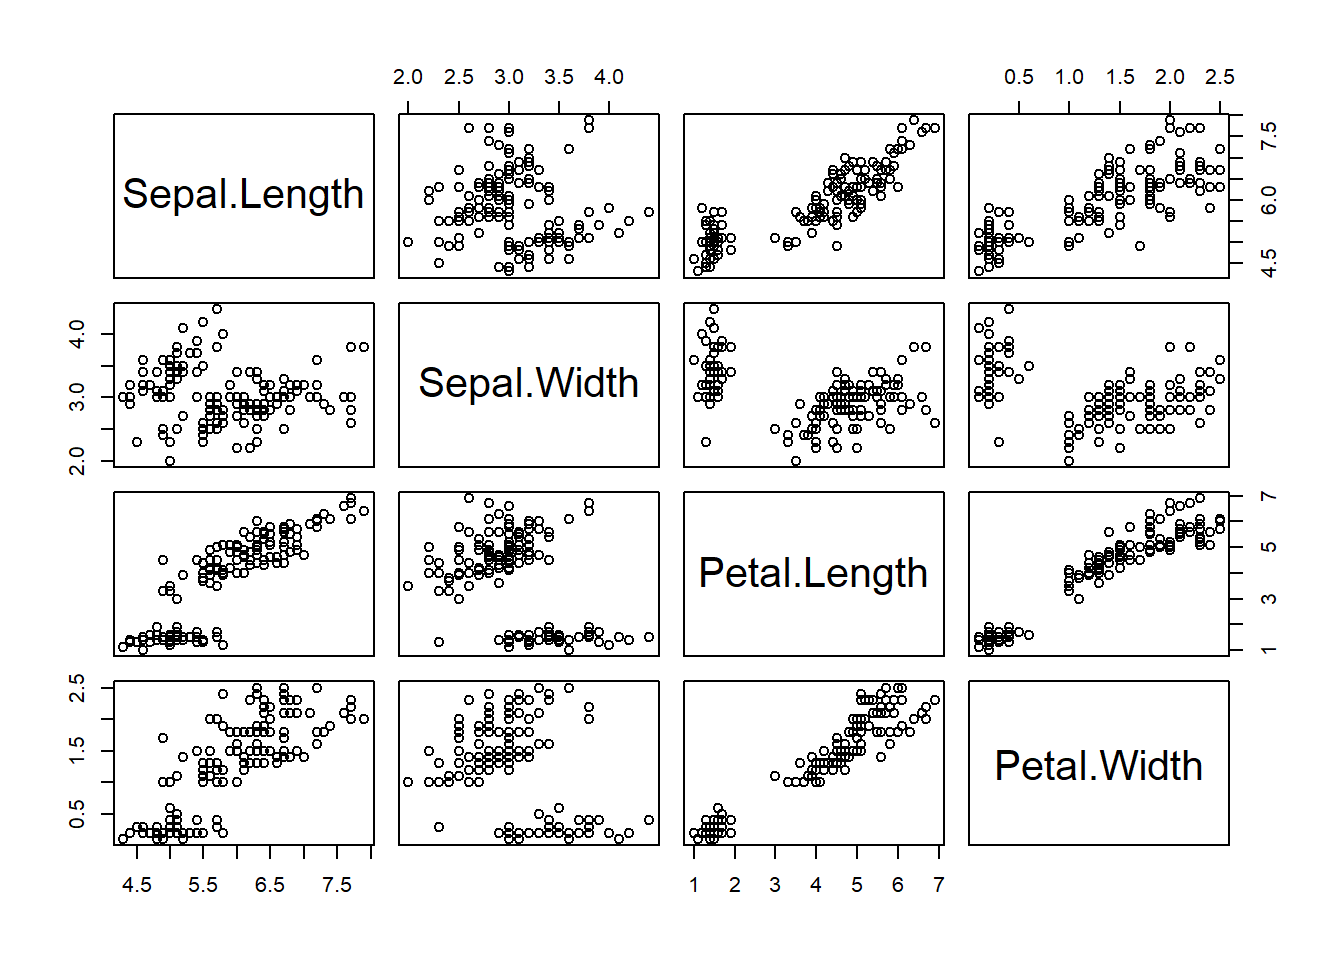
\includegraphics{final_project_files/figure-latex/unnamed-chunk-2-1.pdf}

\textbf{Fig.1 istribution of the study sites and their measured N2O
emissions as well as the archaeal-nitrifier/denitrifier ratio (archaeal
amoA/(nirK + nirS))}

Typographical symbols (+, ×, or ✱) denote average N2O fluxes per site,
the filled/open round, square, and triangle shapes represent different
land-use types, and shape color shows the archaeal-nitrifier/denitrifier
ratio based on the absolute abundance of gene copies determined by qPCR
(n = 72 independent sites).

\hypertarget{relationships-of-global-n2o-fluxes-to-microbial-diversity-and-taxa}{%
\subsubsection{\texorpdfstring{\textbf{Relationships of Global N2O
Fluxes to Microbial Diversity and
Taxa}}{Relationships of Global N2O Fluxes to Microbial Diversity and Taxa}}\label{relationships-of-global-n2o-fluxes-to-microbial-diversity-and-taxa}}

\begin{itemize}
\tightlist
\item
  Microbial diversity varies with latitude: Archaeal diversity increases
  toward the equator, while bacterial diversity is highest in
  mid-latitudes.
\item
  Soil variables affect microbial diversity: Climate and soil conditions
  (like pH, C/N ratio) greatly influence microbial diversity.
\item
  Archaeal diversity linked to N2O emissions: The presence of archaea
  (specifically AOA from Thaumarchaeota) correlates strongly with N2O
  emissions.
\item
  Key microbial groups: The most abundant phyla in global wetlands are
  Proteobacteria, Acidobacteriota, and Chloroflexi, but they aren't
  strongly related to N2O emissions.
\item
  Functional microbes linked to N2O: Specific archaeal groups (like
  Nitrosotenuis and Nitrosocosmicus) are more strongly associated with
  N2O fluxes.
\end{itemize}

\begin{Shaded}
\begin{Highlighting}[]
\CommentTok{\#data}
\NormalTok{data\_1b }\OtherTok{\textless{}{-}} \FunctionTok{read\_excel}\NormalTok{(}\StringTok{"D:/hpliu/Mikk\_dataset/Source\_data.xlsx"}\NormalTok{, }\AttributeTok{sheet =} \StringTok{"Fig1b{-}d"}\NormalTok{)}
\end{Highlighting}
\end{Shaded}

\begin{verbatim}
## New names:
## * `` -> `...1`
\end{verbatim}

\begin{Shaded}
\begin{Highlighting}[]
\FunctionTok{head}\NormalTok{(data\_1b)}
\end{Highlighting}
\end{Shaded}

\begin{verbatim}
## # A tibble: 6 x 6
##   ...1  Site                  Latitude    N2O Archaeal_amoA         nir
##   <chr> <chr>                    <dbl>  <dbl>         <dbl>       <dbl>
## 1 Y001  Iceland_fen_1             64.3 -0.371       402159. 4500024495.
## 2 Y002  Iceland_fen_1             64.3 -1.51         15743. 1193072309.
## 3 Y003  Iceland_fen_1             64.3  1.49         49635. 3633016615.
## 4 Y004  Iceland_fen_1             64.3  0            87676. 8526838441.
## 5 Y005  Iceland_drained_fen_2     64.3 -3.48        415234. 9776754909.
## 6 Y006  Iceland_drained_fen_2     64.3  0            48674. 1113960206.
\end{verbatim}

\begin{Shaded}
\begin{Highlighting}[]
\NormalTok{data\_1bv2 }\OtherTok{\textless{}{-}}\NormalTok{ data\_1b  }\SpecialCharTok{\%\textgreater{}\%}
  \FunctionTok{mutate}\NormalTok{(}\AttributeTok{LogN2O =} \FunctionTok{log10}\NormalTok{(}\DecValTok{15} \SpecialCharTok{+}\NormalTok{ N2O)) }\CommentTok{\# calculate}
\FunctionTok{head}\NormalTok{(data\_1bv2)}
\end{Highlighting}
\end{Shaded}

\begin{verbatim}
## # A tibble: 6 x 7
##   ...1  Site                  Latitude    N2O Archaeal_amoA         nir LogN2O
##   <chr> <chr>                    <dbl>  <dbl>         <dbl>       <dbl>  <dbl>
## 1 Y001  Iceland_fen_1             64.3 -0.371       402159. 4500024495.   1.17
## 2 Y002  Iceland_fen_1             64.3 -1.51         15743. 1193072309.   1.13
## 3 Y003  Iceland_fen_1             64.3  1.49         49635. 3633016615.   1.22
## 4 Y004  Iceland_fen_1             64.3  0            87676. 8526838441.   1.18
## 5 Y005  Iceland_drained_fen_2     64.3 -3.48        415234. 9776754909.   1.06
## 6 Y006  Iceland_drained_fen_2     64.3  0            48674. 1113960206.   1.18
\end{verbatim}

\begin{Shaded}
\begin{Highlighting}[]
\CommentTok{\# standard error (SE) }
\NormalTok{data\_1bv3 }\OtherTok{\textless{}{-}}\NormalTok{ data\_1bv2 }\SpecialCharTok{\%\textgreater{}\%}
  \FunctionTok{group\_by}\NormalTok{(Latitude) }\SpecialCharTok{\%\textgreater{}\%}
  \FunctionTok{summarise}\NormalTok{(}
    \AttributeTok{mean\_LogN2O =} \FunctionTok{mean}\NormalTok{(LogN2O, }\AttributeTok{na.rm =} \ConstantTok{TRUE}\NormalTok{),}
    \AttributeTok{se\_LogN2O =} \FunctionTok{sd}\NormalTok{(LogN2O, }\AttributeTok{na.rm =} \ConstantTok{TRUE}\NormalTok{) }\SpecialCharTok{/} \FunctionTok{sqrt}\NormalTok{(}\FunctionTok{n}\NormalTok{())}
\NormalTok{  )}
\FunctionTok{summary}\NormalTok{(data\_1bv3)}
\end{Highlighting}
\end{Shaded}

\begin{verbatim}
##     Latitude        mean_LogN2O      se_LogN2O       
##  Min.   : 0.9337   Min.   :1.113   Min.   :0.000000  
##  1st Qu.:20.6108   1st Qu.:1.175   1st Qu.:0.005311  
##  Median :38.0169   Median :1.250   Median :0.020408  
##  Mean   :34.2176   Mean   :1.454   Mean   :0.094612  
##  3rd Qu.:48.4935   3rd Qu.:1.630   3rd Qu.:0.108679  
##  Max.   :67.9978   Max.   :2.847   Max.   :1.075233  
##                                    NA's   :21
\end{verbatim}

\begin{Shaded}
\begin{Highlighting}[]
\NormalTok{data\_1bv4 }\OtherTok{\textless{}{-}} \FunctionTok{lm}\NormalTok{(mean\_LogN2O }\SpecialCharTok{\textasciitilde{}}\NormalTok{ Latitude, }\AttributeTok{data =}\NormalTok{ data\_1bv3)}
\NormalTok{data\_1bv4}
\end{Highlighting}
\end{Shaded}

\begin{verbatim}
## 
## Call:
## lm(formula = mean_LogN2O ~ Latitude, data = data_1bv3)
## 
## Coefficients:
## (Intercept)     Latitude  
##     1.84105     -0.01132
\end{verbatim}

\begin{Shaded}
\begin{Highlighting}[]
\FunctionTok{summary}\NormalTok{(data\_1bv4)}
\end{Highlighting}
\end{Shaded}

\begin{verbatim}
## 
## Call:
## lm(formula = mean_LogN2O ~ Latitude, data = data_1bv3)
## 
## Residuals:
##     Min      1Q  Median      3Q     Max 
## -0.6079 -0.1880 -0.0642  0.1485  1.0191 
## 
## Coefficients:
##              Estimate Std. Error t value Pr(>|t|)    
## (Intercept)  1.841055   0.080894   22.76  < 2e-16 ***
## Latitude    -0.011324   0.002059   -5.50 5.64e-07 ***
## ---
## Signif. codes:  0 '***' 0.001 '**' 0.01 '*' 0.05 '.' 0.1 ' ' 1
## 
## Residual standard error: 0.3398 on 71 degrees of freedom
## Multiple R-squared:  0.2988, Adjusted R-squared:  0.2889 
## F-statistic: 30.26 on 1 and 71 DF,  p-value: 5.642e-07
\end{verbatim}

\begin{Shaded}
\begin{Highlighting}[]
\NormalTok{r\_squared }\OtherTok{\textless{}{-}} \FunctionTok{summary}\NormalTok{(data\_1bv4)}\SpecialCharTok{$}\NormalTok{r}


\CommentTok{\# Plot}
\NormalTok{pcPlot\_b}\OtherTok{\textless{}{-}} \FunctionTok{ggplot}\NormalTok{(data\_1bv3, }\FunctionTok{aes}\NormalTok{(}\AttributeTok{x =}\NormalTok{ Latitude, }\AttributeTok{y =}\NormalTok{ mean\_LogN2O)) }\SpecialCharTok{+}
  \FunctionTok{geom\_point}\NormalTok{(}\AttributeTok{color =} \StringTok{"black"}\NormalTok{, }\AttributeTok{size =} \DecValTok{3}\NormalTok{) }\SpecialCharTok{+}  \CommentTok{\# Scatter plot for means}
  \FunctionTok{geom\_errorbar}\NormalTok{(}\FunctionTok{aes}\NormalTok{(}\AttributeTok{ymin =}\NormalTok{ mean\_LogN2O }\SpecialCharTok{{-}}\NormalTok{ se\_LogN2O, }\AttributeTok{ymax =}\NormalTok{ mean\_LogN2O }\SpecialCharTok{+}\NormalTok{ se\_LogN2O), }
                \AttributeTok{width =} \DecValTok{1}\NormalTok{, }\AttributeTok{color =} \StringTok{"black"}\NormalTok{) }\SpecialCharTok{+}  \CommentTok{\# Error bars}
  \FunctionTok{labs}\NormalTok{(}
    \AttributeTok{x =} \StringTok{"Latitude"}\NormalTok{, }
    \AttributeTok{y =} \FunctionTok{expression}\NormalTok{(}\StringTok{"Log"}\NormalTok{[}\DecValTok{10}\NormalTok{] }\SpecialCharTok{*} \StringTok{"15 + N"}\NormalTok{[}\DecValTok{2}\NormalTok{] }\SpecialCharTok{*} \StringTok{"O emission"}\NormalTok{), }
    \AttributeTok{title =} \FunctionTok{expression}\NormalTok{(}\StringTok{"N"}\NormalTok{[}\DecValTok{2}\NormalTok{] }\SpecialCharTok{*} \StringTok{"O emission"}\NormalTok{)}
\NormalTok{  ) }\SpecialCharTok{+}
  \FunctionTok{theme\_classic}\NormalTok{() }\SpecialCharTok{+}
  \FunctionTok{theme}\NormalTok{(}
    \AttributeTok{panel.border =} \FunctionTok{element\_rect}\NormalTok{(}\AttributeTok{color =} \StringTok{"black"}\NormalTok{, }\AttributeTok{fill =} \ConstantTok{NA}\NormalTok{, }\AttributeTok{size =} \FloatTok{0.5}\NormalTok{)}
\NormalTok{  )}\SpecialCharTok{+}
  \FunctionTok{scale\_x\_continuous}\NormalTok{(}
    \AttributeTok{limits =} \FunctionTok{c}\NormalTok{(}\DecValTok{0}\NormalTok{, }\DecValTok{70}\NormalTok{),      }
    \AttributeTok{breaks =} \FunctionTok{seq}\NormalTok{(}\DecValTok{0}\NormalTok{, }\DecValTok{70}\NormalTok{, }\DecValTok{10}\NormalTok{),}
    \AttributeTok{expand =} \FunctionTok{c}\NormalTok{(}\FloatTok{0.01}\NormalTok{, }\FloatTok{0.01}\NormalTok{)}
\NormalTok{    )}
\NormalTok{pcPlot\_b}
\end{Highlighting}
\end{Shaded}

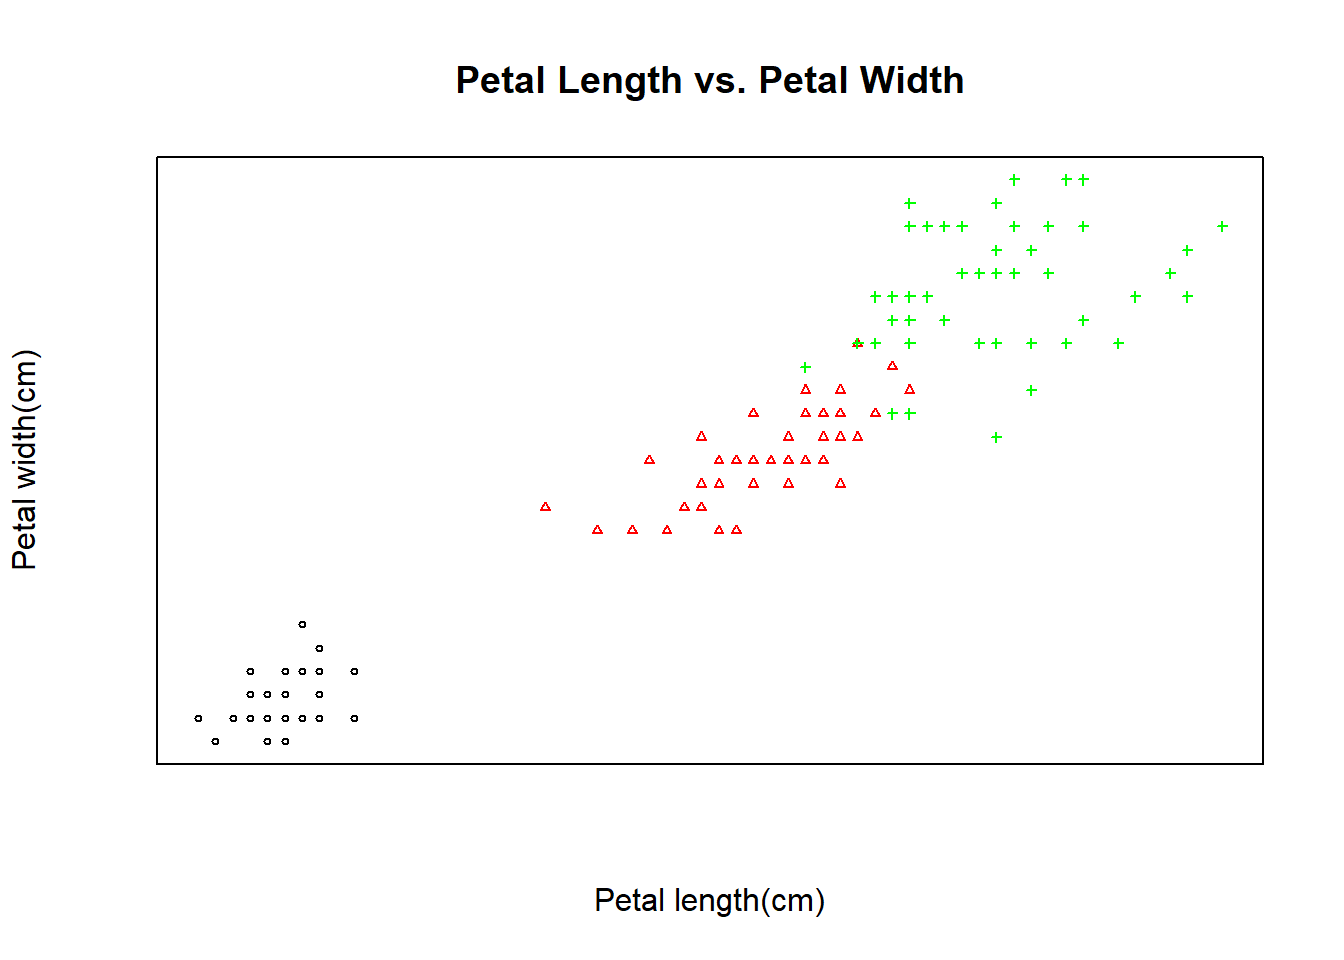
\includegraphics{final_project_files/figure-latex/unnamed-chunk-3-1.pdf}

\begin{Shaded}
\begin{Highlighting}[]
\NormalTok{plot\_b }\OtherTok{\textless{}{-}}\NormalTok{ pcPlot\_b}\SpecialCharTok{+}
  \FunctionTok{stat\_smooth}\NormalTok{(}\AttributeTok{method=}\StringTok{"gam"}\NormalTok{, }\AttributeTok{color =} \StringTok{"red"}\NormalTok{)}\SpecialCharTok{+}
  \FunctionTok{annotate}\NormalTok{(}\StringTok{"text"}\NormalTok{, }
           \AttributeTok{x =} \DecValTok{35}\NormalTok{, }\AttributeTok{y =} \DecValTok{3}\NormalTok{,}
           \AttributeTok{label =} \FunctionTok{paste}\NormalTok{(}\StringTok{"r2 = 0.29"}\NormalTok{, }\StringTok{"}\SpecialCharTok{\textbackslash{}n}\StringTok{ p = 5.642e{-}07"}\NormalTok{), }
           \AttributeTok{size =} \DecValTok{5}\NormalTok{, }\AttributeTok{color =} \StringTok{"black"}\NormalTok{, }\AttributeTok{hjust =} \DecValTok{0}\NormalTok{)}
\NormalTok{plot\_b}
\end{Highlighting}
\end{Shaded}

\begin{verbatim}
## `geom_smooth()` using formula = 'y ~ s(x, bs = "cs")'
\end{verbatim}

\includegraphics{final_project_files/figure-latex/unnamed-chunk-3-2.pdf}

\begin{Shaded}
\begin{Highlighting}[]
\CommentTok{\#c}
\CommentTok{\#data}
\NormalTok{data\_1c }\OtherTok{\textless{}{-}} \FunctionTok{read\_excel}\NormalTok{(}\StringTok{"D:/hpliu/Mikk\_dataset/Source\_data.xlsx"}\NormalTok{, }\AttributeTok{sheet =} \StringTok{"Fig1b{-}d"}\NormalTok{)}
\end{Highlighting}
\end{Shaded}

\begin{verbatim}
## New names:
## * `` -> `...1`
\end{verbatim}

\begin{Shaded}
\begin{Highlighting}[]
\FunctionTok{head}\NormalTok{(data\_1c)}
\end{Highlighting}
\end{Shaded}

\begin{verbatim}
## # A tibble: 6 x 6
##   ...1  Site                  Latitude    N2O Archaeal_amoA         nir
##   <chr> <chr>                    <dbl>  <dbl>         <dbl>       <dbl>
## 1 Y001  Iceland_fen_1             64.3 -0.371       402159. 4500024495.
## 2 Y002  Iceland_fen_1             64.3 -1.51         15743. 1193072309.
## 3 Y003  Iceland_fen_1             64.3  1.49         49635. 3633016615.
## 4 Y004  Iceland_fen_1             64.3  0            87676. 8526838441.
## 5 Y005  Iceland_drained_fen_2     64.3 -3.48        415234. 9776754909.
## 6 Y006  Iceland_drained_fen_2     64.3  0            48674. 1113960206.
\end{verbatim}

\begin{Shaded}
\begin{Highlighting}[]
\NormalTok{data\_1cv2 }\OtherTok{\textless{}{-}}\NormalTok{ data\_1c  }\SpecialCharTok{\%\textgreater{}\%}
  \FunctionTok{mutate}\NormalTok{(}\AttributeTok{LogN2OA =} \FunctionTok{log10}\NormalTok{(}\DecValTok{15} \SpecialCharTok{+}\NormalTok{ Archaeal\_amoA)) }\CommentTok{\# calculate}
\FunctionTok{head}\NormalTok{(data\_1cv2)}
\end{Highlighting}
\end{Shaded}

\begin{verbatim}
## # A tibble: 6 x 7
##   ...1  Site                  Latitude    N2O Archaeal_amoA         nir LogN2OA
##   <chr> <chr>                    <dbl>  <dbl>         <dbl>       <dbl>   <dbl>
## 1 Y001  Iceland_fen_1             64.3 -0.371       402159. 4500024495.    5.60
## 2 Y002  Iceland_fen_1             64.3 -1.51         15743. 1193072309.    4.20
## 3 Y003  Iceland_fen_1             64.3  1.49         49635. 3633016615.    4.70
## 4 Y004  Iceland_fen_1             64.3  0            87676. 8526838441.    4.94
## 5 Y005  Iceland_drained_fen_2     64.3 -3.48        415234. 9776754909.    5.62
## 6 Y006  Iceland_drained_fen_2     64.3  0            48674. 1113960206.    4.69
\end{verbatim}

\begin{Shaded}
\begin{Highlighting}[]
\CommentTok{\# standard error (SE) }
\NormalTok{data\_1cv3 }\OtherTok{\textless{}{-}}\NormalTok{ data\_1cv2 }\SpecialCharTok{\%\textgreater{}\%}
  \FunctionTok{group\_by}\NormalTok{(Latitude) }\SpecialCharTok{\%\textgreater{}\%}
  \FunctionTok{summarise}\NormalTok{(}
    \AttributeTok{mean\_LogN2OA =} \FunctionTok{mean}\NormalTok{(LogN2OA, }\AttributeTok{na.rm =} \ConstantTok{TRUE}\NormalTok{),}
    \AttributeTok{se\_LogN2OA =} \FunctionTok{sd}\NormalTok{(LogN2OA, }\AttributeTok{na.rm =} \ConstantTok{TRUE}\NormalTok{) }\SpecialCharTok{/} \FunctionTok{sqrt}\NormalTok{(}\FunctionTok{n}\NormalTok{())}
\NormalTok{  )}
\FunctionTok{summary}\NormalTok{(data\_1cv3)}
\end{Highlighting}
\end{Shaded}

\begin{verbatim}
##     Latitude        mean_LogN2OA     se_LogN2OA     
##  Min.   : 0.9337   Min.   :1.176   Min.   :0.01018  
##  1st Qu.:20.6108   1st Qu.:5.705   1st Qu.:0.11726  
##  Median :38.0169   Median :7.011   Median :0.25109  
##  Mean   :34.2176   Mean   :6.478   Mean   :0.44104  
##  3rd Qu.:48.4935   3rd Qu.:7.953   3rd Qu.:0.48991  
##  Max.   :67.9978   Max.   :8.763   Max.   :3.41032  
##                                    NA's   :21
\end{verbatim}

\begin{Shaded}
\begin{Highlighting}[]
\NormalTok{data\_1cv4 }\OtherTok{\textless{}{-}} \FunctionTok{lm}\NormalTok{(mean\_LogN2OA }\SpecialCharTok{\textasciitilde{}}\NormalTok{ Latitude, }\AttributeTok{data =}\NormalTok{ data\_1cv3)}
\NormalTok{data\_1cv4}
\end{Highlighting}
\end{Shaded}

\begin{verbatim}
## 
## Call:
## lm(formula = mean_LogN2OA ~ Latitude, data = data_1cv3)
## 
## Coefficients:
## (Intercept)     Latitude  
##     7.97054     -0.04363
\end{verbatim}

\begin{Shaded}
\begin{Highlighting}[]
\FunctionTok{summary}\NormalTok{(data\_1cv4)}
\end{Highlighting}
\end{Shaded}

\begin{verbatim}
## 
## Call:
## lm(formula = mean_LogN2OA ~ Latitude, data = data_1cv3)
## 
## Residuals:
##     Min      1Q  Median      3Q     Max 
## -4.9270 -0.8265  0.2265  1.1263  2.5834 
## 
## Coefficients:
##             Estimate Std. Error t value Pr(>|t|)    
## (Intercept)  7.97054    0.38036  20.955  < 2e-16 ***
## Latitude    -0.04363    0.00968  -4.507 2.53e-05 ***
## ---
## Signif. codes:  0 '***' 0.001 '**' 0.01 '*' 0.05 '.' 0.1 ' ' 1
## 
## Residual standard error: 1.598 on 71 degrees of freedom
## Multiple R-squared:  0.2225, Adjusted R-squared:  0.2115 
## F-statistic: 20.31 on 1 and 71 DF,  p-value: 2.528e-05
\end{verbatim}

\begin{Shaded}
\begin{Highlighting}[]
\CommentTok{\# Plot}
\NormalTok{pcPlot\_c }\OtherTok{\textless{}{-}} \FunctionTok{ggplot}\NormalTok{(data\_1cv3, }\FunctionTok{aes}\NormalTok{(}\AttributeTok{x =}\NormalTok{ Latitude, }\AttributeTok{y =}\NormalTok{ mean\_LogN2OA)) }\SpecialCharTok{+}
  \FunctionTok{geom\_point}\NormalTok{(}\AttributeTok{color =} \StringTok{"black"}\NormalTok{, }\AttributeTok{size =} \DecValTok{3}\NormalTok{) }\SpecialCharTok{+}  \CommentTok{\# Scatter plot for means}
  \FunctionTok{geom\_errorbar}\NormalTok{(}\FunctionTok{aes}\NormalTok{(}\AttributeTok{ymin =}\NormalTok{ mean\_LogN2OA }\SpecialCharTok{{-}}\NormalTok{ se\_LogN2OA, }\AttributeTok{ymax =}\NormalTok{ mean\_LogN2OA }\SpecialCharTok{+}\NormalTok{ se\_LogN2OA), }
                \AttributeTok{width =} \DecValTok{1}\NormalTok{, }\AttributeTok{color =} \StringTok{"black"}\NormalTok{) }\SpecialCharTok{+}  \CommentTok{\# Error bars}
  \FunctionTok{labs}\NormalTok{(}
    \AttributeTok{x =} \StringTok{"Latitude"}\NormalTok{, }
    \AttributeTok{y =} \FunctionTok{expression}\NormalTok{(}\StringTok{"Log"}\NormalTok{[}\DecValTok{10}\NormalTok{] }\SpecialCharTok{*} \StringTok{" 15 + Archaeal "} \SpecialCharTok{*} \FunctionTok{italic}\NormalTok{(}\StringTok{" amoA"}\NormalTok{)),}
    \AttributeTok{title =}  \FunctionTok{expression}\NormalTok{(}\StringTok{"Archaeal "}\SpecialCharTok{*} \FunctionTok{italic}\NormalTok{(}\StringTok{"amoA"}\NormalTok{))}
\NormalTok{  ) }\SpecialCharTok{+}
  \FunctionTok{theme\_classic}\NormalTok{() }\SpecialCharTok{+}
  \FunctionTok{theme}\NormalTok{(}
    \AttributeTok{panel.border =} \FunctionTok{element\_rect}\NormalTok{(}\AttributeTok{color =} \StringTok{"black"}\NormalTok{, }\AttributeTok{fill =} \ConstantTok{NA}\NormalTok{, }\AttributeTok{size =} \FloatTok{0.5}\NormalTok{)}
\NormalTok{  )}\SpecialCharTok{+}
  \FunctionTok{scale\_x\_continuous}\NormalTok{(}
    \AttributeTok{limits =} \FunctionTok{c}\NormalTok{(}\DecValTok{0}\NormalTok{, }\DecValTok{70}\NormalTok{),      }
    \AttributeTok{breaks =} \FunctionTok{seq}\NormalTok{(}\DecValTok{0}\NormalTok{, }\DecValTok{70}\NormalTok{, }\DecValTok{10}\NormalTok{),}
    \AttributeTok{expand =} \FunctionTok{c}\NormalTok{(}\FloatTok{0.01}\NormalTok{, }\FloatTok{0.01}\NormalTok{)}
\NormalTok{  )}
\NormalTok{plot\_c }\OtherTok{\textless{}{-}}\NormalTok{ pcPlot\_c}\SpecialCharTok{+}
  \FunctionTok{stat\_smooth}\NormalTok{(}\AttributeTok{method=}\StringTok{"lm"}\NormalTok{, }\AttributeTok{color =} \StringTok{"red"}\NormalTok{)}\SpecialCharTok{+}
  \FunctionTok{annotate}\NormalTok{(}\StringTok{"text"}\NormalTok{, }
           \AttributeTok{x =} \DecValTok{3}\NormalTok{, }\AttributeTok{y =} \DecValTok{3}\NormalTok{,}
           \AttributeTok{label =} \FunctionTok{paste}\NormalTok{(}\StringTok{"r2 = 0.22"}\NormalTok{, }\StringTok{"}\SpecialCharTok{\textbackslash{}n}\StringTok{ p = 2.528e{-}05"}\NormalTok{), }
           \AttributeTok{size =} \DecValTok{5}\NormalTok{, }\AttributeTok{color =} \StringTok{"black"}\NormalTok{, }\AttributeTok{hjust =} \DecValTok{0}\NormalTok{)}
\NormalTok{plot\_c}
\end{Highlighting}
\end{Shaded}

\begin{verbatim}
## `geom_smooth()` using formula = 'y ~ x'
\end{verbatim}

\includegraphics{final_project_files/figure-latex/unnamed-chunk-3-3.pdf}

\begin{Shaded}
\begin{Highlighting}[]
\CommentTok{\#d}
\CommentTok{\#data}
\NormalTok{data\_1d }\OtherTok{\textless{}{-}} \FunctionTok{read\_excel}\NormalTok{(}\StringTok{"D:/hpliu/Mikk\_dataset/Source\_data.xlsx"}\NormalTok{, }\AttributeTok{sheet =} \StringTok{"Fig1b{-}d"}\NormalTok{)}
\end{Highlighting}
\end{Shaded}

\begin{verbatim}
## New names:
## * `` -> `...1`
\end{verbatim}

\begin{Shaded}
\begin{Highlighting}[]
\FunctionTok{head}\NormalTok{(data\_1d)}
\end{Highlighting}
\end{Shaded}

\begin{verbatim}
## # A tibble: 6 x 6
##   ...1  Site                  Latitude    N2O Archaeal_amoA         nir
##   <chr> <chr>                    <dbl>  <dbl>         <dbl>       <dbl>
## 1 Y001  Iceland_fen_1             64.3 -0.371       402159. 4500024495.
## 2 Y002  Iceland_fen_1             64.3 -1.51         15743. 1193072309.
## 3 Y003  Iceland_fen_1             64.3  1.49         49635. 3633016615.
## 4 Y004  Iceland_fen_1             64.3  0            87676. 8526838441.
## 5 Y005  Iceland_drained_fen_2     64.3 -3.48        415234. 9776754909.
## 6 Y006  Iceland_drained_fen_2     64.3  0            48674. 1113960206.
\end{verbatim}

\begin{Shaded}
\begin{Highlighting}[]
\NormalTok{data\_1dv2 }\OtherTok{\textless{}{-}}\NormalTok{ data\_1d  }\SpecialCharTok{\%\textgreater{}\%}
  \FunctionTok{mutate}\NormalTok{(}\AttributeTok{LogN2On =} \FunctionTok{log10}\NormalTok{(}\DecValTok{15} \SpecialCharTok{+}\NormalTok{ nir)) }\CommentTok{\# calculate}
\FunctionTok{head}\NormalTok{(data\_1dv2)}
\end{Highlighting}
\end{Shaded}

\begin{verbatim}
## # A tibble: 6 x 7
##   ...1  Site                  Latitude    N2O Archaeal_amoA         nir LogN2On
##   <chr> <chr>                    <dbl>  <dbl>         <dbl>       <dbl>   <dbl>
## 1 Y001  Iceland_fen_1             64.3 -0.371       402159. 4500024495.    9.65
## 2 Y002  Iceland_fen_1             64.3 -1.51         15743. 1193072309.    9.08
## 3 Y003  Iceland_fen_1             64.3  1.49         49635. 3633016615.    9.56
## 4 Y004  Iceland_fen_1             64.3  0            87676. 8526838441.    9.93
## 5 Y005  Iceland_drained_fen_2     64.3 -3.48        415234. 9776754909.    9.99
## 6 Y006  Iceland_drained_fen_2     64.3  0            48674. 1113960206.    9.05
\end{verbatim}

\begin{Shaded}
\begin{Highlighting}[]
\CommentTok{\# standard error (SE) }
\NormalTok{data\_1dv3 }\OtherTok{\textless{}{-}}\NormalTok{ data\_1dv2 }\SpecialCharTok{\%\textgreater{}\%}
  \FunctionTok{group\_by}\NormalTok{(Latitude) }\SpecialCharTok{\%\textgreater{}\%}
  \FunctionTok{summarise}\NormalTok{(}
    \AttributeTok{mean\_LogN2On =} \FunctionTok{mean}\NormalTok{(LogN2On, }\AttributeTok{na.rm =} \ConstantTok{TRUE}\NormalTok{),}
    \AttributeTok{se\_LogN2On =} \FunctionTok{sd}\NormalTok{(LogN2On, }\AttributeTok{na.rm =} \ConstantTok{TRUE}\NormalTok{) }\SpecialCharTok{/} \FunctionTok{sqrt}\NormalTok{(}\FunctionTok{n}\NormalTok{())}
\NormalTok{  )}
\FunctionTok{summary}\NormalTok{(data\_1dv3)}
\end{Highlighting}
\end{Shaded}

\begin{verbatim}
##     Latitude        mean_LogN2On      se_LogN2On      
##  Min.   : 0.9337   Min.   : 7.079   Min.   :0.005592  
##  1st Qu.:20.6108   1st Qu.: 9.118   1st Qu.:0.063771  
##  Median :38.0169   Median : 9.552   Median :0.110340  
##  Mean   :34.2176   Mean   : 9.479   Mean   :0.152640  
##  3rd Qu.:48.4935   3rd Qu.:10.038   3rd Qu.:0.207970  
##  Max.   :67.9978   Max.   :11.074   Max.   :0.953328  
##                                     NA's   :21
\end{verbatim}

\begin{Shaded}
\begin{Highlighting}[]
\NormalTok{data\_1dv4 }\OtherTok{\textless{}{-}} \FunctionTok{lm}\NormalTok{(mean\_LogN2On }\SpecialCharTok{\textasciitilde{}}\NormalTok{ Latitude, }\AttributeTok{data =}\NormalTok{ data\_1dv3)}
\NormalTok{data\_1dv4}
\end{Highlighting}
\end{Shaded}

\begin{verbatim}
## 
## Call:
## lm(formula = mean_LogN2On ~ Latitude, data = data_1dv3)
## 
## Coefficients:
## (Intercept)     Latitude  
##   9.4575131    0.0006176
\end{verbatim}

\begin{Shaded}
\begin{Highlighting}[]
\FunctionTok{summary}\NormalTok{(data\_1dv4)}
\end{Highlighting}
\end{Shaded}

\begin{verbatim}
## 
## Call:
## lm(formula = mean_LogN2On ~ Latitude, data = data_1dv3)
## 
## Residuals:
##      Min       1Q   Median       3Q      Max 
## -2.40454 -0.34804  0.06402  0.58011  1.58960 
## 
## Coefficients:
##              Estimate Std. Error t value Pr(>|t|)    
## (Intercept) 9.4575131  0.1788228  52.888   <2e-16 ***
## Latitude    0.0006176  0.0045510   0.136    0.892    
## ---
## Signif. codes:  0 '***' 0.001 '**' 0.01 '*' 0.05 '.' 0.1 ' ' 1
## 
## Residual standard error: 0.7511 on 71 degrees of freedom
## Multiple R-squared:  0.0002593,  Adjusted R-squared:  -0.01382 
## F-statistic: 0.01841 on 1 and 71 DF,  p-value: 0.8924
\end{verbatim}

\begin{Shaded}
\begin{Highlighting}[]
\NormalTok{r2\_value\_1 }\OtherTok{\textless{}{-}} \FunctionTok{summary}\NormalTok{(data\_1dv4)}\SpecialCharTok{$}\NormalTok{r.squared}



\CommentTok{\# Plot}
\NormalTok{pcPlot\_d }\OtherTok{\textless{}{-}} \FunctionTok{ggplot}\NormalTok{(data\_1dv3, }\FunctionTok{aes}\NormalTok{(}\AttributeTok{x =}\NormalTok{ Latitude, }\AttributeTok{y =}\NormalTok{ mean\_LogN2On)) }\SpecialCharTok{+}
  \FunctionTok{geom\_point}\NormalTok{(}\AttributeTok{color =} \StringTok{"black"}\NormalTok{, }\AttributeTok{size =} \DecValTok{3}\NormalTok{) }\SpecialCharTok{+}  \CommentTok{\# Scatter plot for means}
  \FunctionTok{geom\_errorbar}\NormalTok{(}\FunctionTok{aes}\NormalTok{(}\AttributeTok{ymin =}\NormalTok{ mean\_LogN2On }\SpecialCharTok{{-}}\NormalTok{ se\_LogN2On, }\AttributeTok{ymax =}\NormalTok{ mean\_LogN2On }\SpecialCharTok{+}\NormalTok{ se\_LogN2On), }
                \AttributeTok{width =} \DecValTok{1}\NormalTok{, }\AttributeTok{color =} \StringTok{"black"}\NormalTok{) }\SpecialCharTok{+}  \CommentTok{\# Error bars}
  \FunctionTok{labs}\NormalTok{(}
    \AttributeTok{x =} \StringTok{"Latitude"}\NormalTok{, }
    \AttributeTok{y =} \FunctionTok{expression}\NormalTok{(}\StringTok{"Log"}\NormalTok{[}\DecValTok{10}\NormalTok{] }\SpecialCharTok{*} \StringTok{" 15 + "} \SpecialCharTok{*} \FunctionTok{italic}\NormalTok{(}\StringTok{"nir"}\NormalTok{)),}
    \AttributeTok{title =}  \FunctionTok{expression}\NormalTok{(}\StringTok{"nir( "}\SpecialCharTok{*} \FunctionTok{italic}\NormalTok{(}\StringTok{"nirK + nirS"}\NormalTok{)}\SpecialCharTok{*}\StringTok{")"}\NormalTok{)}
\NormalTok{  ) }\SpecialCharTok{+}
  \FunctionTok{theme\_classic}\NormalTok{() }\SpecialCharTok{+}
  \FunctionTok{theme}\NormalTok{(}
    \AttributeTok{panel.border =} \FunctionTok{element\_rect}\NormalTok{(}\AttributeTok{color =} \StringTok{"black"}\NormalTok{, }\AttributeTok{fill =} \ConstantTok{NA}\NormalTok{, }\AttributeTok{size =} \FloatTok{0.5}\NormalTok{)}
\NormalTok{  )}\SpecialCharTok{+}
  \FunctionTok{scale\_x\_continuous}\NormalTok{(}
    \AttributeTok{limits =} \FunctionTok{c}\NormalTok{(}\DecValTok{0}\NormalTok{, }\DecValTok{70}\NormalTok{),      }
    \AttributeTok{breaks =} \FunctionTok{seq}\NormalTok{(}\DecValTok{0}\NormalTok{, }\DecValTok{70}\NormalTok{, }\DecValTok{10}\NormalTok{),}
    \AttributeTok{expand =} \FunctionTok{c}\NormalTok{(}\FloatTok{0.01}\NormalTok{, }\FloatTok{0.01}\NormalTok{)}
\NormalTok{  )}
\NormalTok{pcPlot\_d}
\end{Highlighting}
\end{Shaded}

\includegraphics{final_project_files/figure-latex/unnamed-chunk-3-4.pdf}

\begin{Shaded}
\begin{Highlighting}[]
\NormalTok{plot\_d }\OtherTok{\textless{}{-}}\NormalTok{pcPlot\_d }\SpecialCharTok{+}
  \FunctionTok{stat\_smooth}\NormalTok{(}\AttributeTok{method=}\StringTok{"lm"}\NormalTok{, }\AttributeTok{color =} \StringTok{"red"}\NormalTok{)}\SpecialCharTok{+}
  \FunctionTok{annotate}\NormalTok{(}\StringTok{"text"}\NormalTok{, }
           \AttributeTok{x =} \DecValTok{3}\NormalTok{, }\AttributeTok{y =} \DecValTok{7}\NormalTok{,}
           \AttributeTok{label =} \FunctionTok{paste}\NormalTok{(}\StringTok{"r2 = 0.0002"}\NormalTok{, }\StringTok{"}\SpecialCharTok{\textbackslash{}n}\StringTok{ p = 0.8924"}\NormalTok{), }
           \AttributeTok{size =} \DecValTok{5}\NormalTok{, }\AttributeTok{color =} \StringTok{"black"}\NormalTok{, }\AttributeTok{hjust =} \DecValTok{0}\NormalTok{)}
\NormalTok{plot\_d}
\end{Highlighting}
\end{Shaded}

\begin{verbatim}
## `geom_smooth()` using formula = 'y ~ x'
\end{verbatim}

\includegraphics{final_project_files/figure-latex/unnamed-chunk-3-5.pdf}

\begin{Shaded}
\begin{Highlighting}[]
\CommentTok{\#combine}
\FunctionTok{library}\NormalTok{(cowplot)}
\end{Highlighting}
\end{Shaded}

\begin{verbatim}
## Warning: 套件 'cowplot' 是用 R 版本 4.4.2 來建造的
\end{verbatim}

\begin{Shaded}
\begin{Highlighting}[]
\NormalTok{combined\_plot}\OtherTok{\textless{}{-}}\FunctionTok{plot\_grid}\NormalTok{(plot\_b, plot\_c, plot\_d, }
          \AttributeTok{ncol =} \DecValTok{3}\NormalTok{,   }
          \AttributeTok{nrow =} \DecValTok{1}\NormalTok{,   }
          \AttributeTok{rel\_widths =} \FunctionTok{c}\NormalTok{(}\DecValTok{1}\NormalTok{, }\DecValTok{1}\NormalTok{, }\DecValTok{1}\NormalTok{)  }
\NormalTok{          )}
\end{Highlighting}
\end{Shaded}

\begin{verbatim}
## `geom_smooth()` using formula = 'y ~ s(x, bs = "cs")'
## `geom_smooth()` using formula = 'y ~ x'
## `geom_smooth()` using formula = 'y ~ x'
\end{verbatim}

\begin{Shaded}
\begin{Highlighting}[]
\FunctionTok{plot}\NormalTok{(combined\_plot)}
\end{Highlighting}
\end{Shaded}

\includegraphics{final_project_files/figure-latex/unnamed-chunk-3-6.pdf}

\textbf{Fig.2 atitudinal gradient of N2O emissions, archaeal amoA and
nir (nirK+nirS)}

Error bars represent the standard error (SE) of the means (n=74
independent sites). The statistical test used was two-sided.

\hypertarget{metagenomic-analysis-of-pathways-underlying-global-n2o-fluxes}{%
\subsubsection{\texorpdfstring{\textbf{Metagenomic Analysis of Pathways
Underlying Global N2O
Fluxes}}{Metagenomic Analysis of Pathways Underlying Global N2O Fluxes}}\label{metagenomic-analysis-of-pathways-underlying-global-n2o-fluxes}}

\begin{itemize}
\tightlist
\item
  Key genes involved in N2O production: Archaeal amoA gene (linked to
  ammonia oxidation) strongly correlates with N2O emission.
\item
  Ammonia oxidation pathway: Thaumarchaeota, including Nitrososphaera
  and Nitrosocosmicus, are crucial for ammonia oxidation and N2O
  emission.
\item
  Genomic analysis supports findings: A comparison of archaeal genomes
  shows that ammonia-oxidizing archaea are more abundant than bacteria
  in wetland soils.
\end{itemize}

\hypertarget{functional-genes-driving-global-n2o-fluxes}{%
\subsubsection{\texorpdfstring{\textbf{Functional Genes Driving Global
N2O
Fluxes}}{Functional Genes Driving Global N2O Fluxes}}\label{functional-genes-driving-global-n2o-fluxes}}

\begin{itemize}
\tightlist
\item
  qPCR findings: Archaeal and bacterial amoA genes are the most strongly
  correlated with N2O emissions.
\item
  Nitrification plays a key role: Archaeal nitrifiers (rather than
  denitrifiers) dominate in lower latitudes and contribute more to N2O
  emissions.
\item
  \textbf{Gene diversity and N2O emissions}: Higher diversity of N
  cycle-related genes is associated with higher N2O emissions.
\item
  Denitrification genes: Genes for denitrification (like nir and nosZ)
  show weaker correlations with N2O emissions.
\end{itemize}

\begin{Shaded}
\begin{Highlighting}[]
\FunctionTok{library}\NormalTok{(corrplot)}
\end{Highlighting}
\end{Shaded}

\begin{verbatim}
## Warning: 套件 'corrplot' 是用 R 版本 4.4.2 來建造的
\end{verbatim}

\begin{verbatim}
## corrplot 0.95 loaded
\end{verbatim}

\begin{Shaded}
\begin{Highlighting}[]
\FunctionTok{library}\NormalTok{(reshape)}
\end{Highlighting}
\end{Shaded}

\begin{verbatim}
## Warning: 套件 'reshape' 是用 R 版本 4.4.2 來建造的
\end{verbatim}

\begin{verbatim}
## 
## 載入套件:'reshape'
\end{verbatim}

\begin{verbatim}
## 下列物件被遮斷自 'package:cowplot':
## 
##     stamp
\end{verbatim}

\begin{verbatim}
## 下列物件被遮斷自 'package:dplyr':
## 
##     rename
\end{verbatim}

\begin{Shaded}
\begin{Highlighting}[]
\FunctionTok{library}\NormalTok{(RColorBrewer)}

\NormalTok{data\_4 }\OtherTok{\textless{}{-}} \FunctionTok{read\_excel}\NormalTok{(}\StringTok{"D:/hpliu/Mikk\_dataset/Source\_data.xlsx"}\NormalTok{, }\AttributeTok{sheet =} \StringTok{"Fig4a"}\NormalTok{)}
\end{Highlighting}
\end{Shaded}

\begin{verbatim}
## New names:
## * `` -> `...1`
\end{verbatim}

\begin{Shaded}
\begin{Highlighting}[]
\FunctionTok{head}\NormalTok{(data\_4)}
\end{Highlighting}
\end{Shaded}

\begin{verbatim}
## # A tibble: 6 x 19
##   ...1          N2O Latitude pH    VPG     OrM Water_content    NO3    NH4 `C/N`
##   <chr>       <dbl>    <dbl> <chr> <chr> <dbl>         <dbl>  <dbl>  <dbl> <chr>
## 1 Bashkortos~  1.27    55.5  6.75~ 5     0.29          0.351 0.876  -0.595 1.10~
## 2 Bashkortos~  1.47    55.4  4.45~ 5     0.342         0.209 1.11    1.50  NA   
## 3 Bashkortos~  2.19    55.4  3.82~ 5     0.29          0.418 1.01    1.06  1.06~
## 4 Bashkortos~  1.17    55.5  6.14~ 1     0.507         0.93  0.0780  1.66  1.24~
## 5 Borneo_dra~  2.43     5.32 2.16~ 4.75  0.784         0.384 1.15    1.69  1.46~
## 6 Borneo_swa~  1.95     5.32 2.30~ 5     0.793         0.610 1.50    1.66  1.35~
## # i 9 more variables: Water_table <chr>, MAT <dbl>, MAP <dbl>, nirK <dbl>,
## #   nirS <dbl>, nosZI <dbl>, nosZII <dbl>, Bacterial_amoA <dbl>,
## #   Archaeal_amoA <dbl>
\end{verbatim}

\begin{Shaded}
\begin{Highlighting}[]
\NormalTok{numeric\_data }\OtherTok{\textless{}{-}}\NormalTok{ data\_4 }\SpecialCharTok{\%\textgreater{}\%} \FunctionTok{select}\NormalTok{(}\FunctionTok{where}\NormalTok{(is.numeric))}
\NormalTok{M}\OtherTok{\textless{}{-}}\FunctionTok{cor}\NormalTok{(numeric\_data)}
\FunctionTok{head}\NormalTok{(}\FunctionTok{round}\NormalTok{(M,}\DecValTok{2}\NormalTok{))}
\end{Highlighting}
\end{Shaded}

\begin{verbatim}
##                 N2O Latitude   OrM Water_content   NO3   NH4   MAT   MAP  nirK
## N2O            1.00    -0.48 -0.07         -0.26  0.45  0.14  0.37  0.19  0.02
## Latitude      -0.48     1.00  0.36          0.08 -0.25 -0.17 -0.81 -0.55 -0.02
## OrM           -0.07     0.36  1.00          0.14  0.10  0.09 -0.47 -0.15  0.24
## Water_content -0.26     0.08  0.14          1.00 -0.46  0.19 -0.12  0.00  0.13
## NO3            0.45    -0.25  0.10         -0.46  1.00 -0.01  0.19  0.11  0.15
## NH4            0.14    -0.17  0.09          0.19 -0.01  1.00  0.08  0.18  0.13
##                nirS nosZI nosZII Bacterial_amoA Archaeal_amoA
## N2O            0.12  0.09   0.26           0.13          0.37
## Latitude      -0.26 -0.18  -0.29           0.20         -0.43
## OrM           -0.41  0.00  -0.32           0.02         -0.35
## Water_content -0.08  0.05  -0.14          -0.20         -0.29
## NO3            0.25  0.15   0.28           0.43          0.40
## NH4            0.00  0.20   0.08          -0.06         -0.05
\end{verbatim}

\begin{Shaded}
\begin{Highlighting}[]
\FunctionTok{corrplot}\NormalTok{(M, }\AttributeTok{type=}\StringTok{"upper"}\NormalTok{, }\AttributeTok{order=}\StringTok{"hclust"}\NormalTok{, }\AttributeTok{tl.col=}\StringTok{"black"}\NormalTok{, }\AttributeTok{tl.srt=}\DecValTok{40}\NormalTok{,}
         \AttributeTok{col=}\FunctionTok{brewer.pal}\NormalTok{(}\AttributeTok{n=}\DecValTok{8}\NormalTok{, }\AttributeTok{name=}\StringTok{"RdBu"}\NormalTok{))}
\end{Highlighting}
\end{Shaded}

\includegraphics{final_project_files/figure-latex/unnamed-chunk-4-1.pdf}

\textbf{Fig.3 rogen-cycle genes as the main factors explaining N2O
emissions across the global wetland soils. a Correlations between
environmental}

variables, the abundance of nir, nosZ and amoA genes (quantified by
qPCR) and N2O emission (n = 74). The abbreviations are archaeal amoA
(arch-amoA), bacterial amoA (bac-amoA), organic matter (OrM), pH (soil
pH), C/N (soil carbon to nitrogen ratio), Von Post grade of
decomposition (VPG).

\hypertarget{environmental-determinants-of-n2o-related-microbial-communities}{%
\subsubsection{\texorpdfstring{\textbf{Environmental Determinants of
N2O-Related Microbial
Communities}}{Environmental Determinants of N2O-Related Microbial Communities}}\label{environmental-determinants-of-n2o-related-microbial-communities}}

\begin{itemize}
\tightlist
\item
  Soil temperature impacts AOA: Archaeal amoA activity peaks around
  20°C, suggesting that warmer soil temperatures can enhance N2O
  emissions through increased AOA abundance.
\item
  AOA/AOB ratio: A higher ratio of AOA to AOB (ammonia-oxidizing
  bacteria) is positively correlated with soil temperature.
\end{itemize}

\begin{Shaded}
\begin{Highlighting}[]
\NormalTok{data\_1 }\OtherTok{\textless{}{-}} \FunctionTok{read\_excel}\NormalTok{(}\StringTok{"D:/hpliu/Mikk\_dataset/Source\_data.xlsx"}\NormalTok{, }\AttributeTok{sheet =} \StringTok{"EDFig.1"}\NormalTok{)}
\end{Highlighting}
\end{Shaded}

\begin{verbatim}
## New names:
## * `` -> `...1`
\end{verbatim}

\begin{Shaded}
\begin{Highlighting}[]
\FunctionTok{head}\NormalTok{(data\_1)}
\end{Highlighting}
\end{Shaded}

\begin{verbatim}
## # A tibble: 6 x 8
##   ...1  Site          N2O Max_temperature_of_w~1 Agricultural_intensity Land_use
##   <chr> <chr>       <dbl>                  <dbl>                  <dbl> <chr>   
## 1 Y001  Iceland_f~ -0.371                   11.2                      1 fen     
## 2 Y002  Iceland_f~ -1.51                    11.2                      1 fen     
## 3 Y003  Iceland_f~  1.49                    11.2                      1 fen     
## 4 Y004  Iceland_f~  0                       11.2                      1 fen     
## 5 Y005  Iceland_d~ -3.48                    11.8                      1 pasture 
## 6 Y006  Iceland_d~  0                       11.8                      1 pasture 
## # i abbreviated name: 1: Max_temperature_of_warmest_month
## # i 2 more variables: Longitude <dbl>, Latitude <dbl>
\end{verbatim}

\begin{Shaded}
\begin{Highlighting}[]
\NormalTok{data\_1v21 }\OtherTok{\textless{}{-}}\NormalTok{ data\_1  }\SpecialCharTok{\%\textgreater{}\%}
  \FunctionTok{mutate}\NormalTok{(}\AttributeTok{Biome\_type =} \FunctionTok{ifelse}\NormalTok{(data\_1}\SpecialCharTok{$}\NormalTok{Latitude }\SpecialCharTok{\textgreater{}=} \SpecialCharTok{{-}}\FloatTok{23.5} \SpecialCharTok{\&}\NormalTok{ data\_1}\SpecialCharTok{$}\NormalTok{Latitude }\SpecialCharTok{\textless{}=} \FloatTok{23.5}\NormalTok{, }\StringTok{"Tropical"}\NormalTok{, }\StringTok{"Non{-}Tropical"}\NormalTok{))}
\FunctionTok{head}\NormalTok{(data\_1v21)}
\end{Highlighting}
\end{Shaded}

\begin{verbatim}
## # A tibble: 6 x 9
##   ...1  Site          N2O Max_temperature_of_w~1 Agricultural_intensity Land_use
##   <chr> <chr>       <dbl>                  <dbl>                  <dbl> <chr>   
## 1 Y001  Iceland_f~ -0.371                   11.2                      1 fen     
## 2 Y002  Iceland_f~ -1.51                    11.2                      1 fen     
## 3 Y003  Iceland_f~  1.49                    11.2                      1 fen     
## 4 Y004  Iceland_f~  0                       11.2                      1 fen     
## 5 Y005  Iceland_d~ -3.48                    11.8                      1 pasture 
## 6 Y006  Iceland_d~  0                       11.8                      1 pasture 
## # i abbreviated name: 1: Max_temperature_of_warmest_month
## # i 3 more variables: Longitude <dbl>, Latitude <dbl>, Biome_type <chr>
\end{verbatim}

\begin{Shaded}
\begin{Highlighting}[]
\NormalTok{data\_1v2 }\OtherTok{\textless{}{-}}\NormalTok{ data\_1v21  }\SpecialCharTok{\%\textgreater{}\%}
  \FunctionTok{mutate}\NormalTok{(}\AttributeTok{LogN2Oe =} \FunctionTok{log10}\NormalTok{(}\DecValTok{15} \SpecialCharTok{+}\NormalTok{ N2O)) }\CommentTok{\# calculate}
\FunctionTok{head}\NormalTok{(data\_1v2)}
\end{Highlighting}
\end{Shaded}

\begin{verbatim}
## # A tibble: 6 x 10
##   ...1  Site          N2O Max_temperature_of_w~1 Agricultural_intensity Land_use
##   <chr> <chr>       <dbl>                  <dbl>                  <dbl> <chr>   
## 1 Y001  Iceland_f~ -0.371                   11.2                      1 fen     
## 2 Y002  Iceland_f~ -1.51                    11.2                      1 fen     
## 3 Y003  Iceland_f~  1.49                    11.2                      1 fen     
## 4 Y004  Iceland_f~  0                       11.2                      1 fen     
## 5 Y005  Iceland_d~ -3.48                    11.8                      1 pasture 
## 6 Y006  Iceland_d~  0                       11.8                      1 pasture 
## # i abbreviated name: 1: Max_temperature_of_warmest_month
## # i 4 more variables: Longitude <dbl>, Latitude <dbl>, Biome_type <chr>,
## #   LogN2Oe <dbl>
\end{verbatim}

\begin{Shaded}
\begin{Highlighting}[]
\NormalTok{data\_1v2}
\end{Highlighting}
\end{Shaded}

\begin{verbatim}
## # A tibble: 196 x 10
##    ...1  Site         N2O Max_temperature_of_w~1 Agricultural_intensity Land_use
##    <chr> <chr>      <dbl>                  <dbl>                  <dbl> <chr>   
##  1 Y001  Iceland_~ -0.371                   11.2                      1 fen     
##  2 Y002  Iceland_~ -1.51                    11.2                      1 fen     
##  3 Y003  Iceland_~  1.49                    11.2                      1 fen     
##  4 Y004  Iceland_~  0                       11.2                      1 fen     
##  5 Y005  Iceland_~ -3.48                    11.8                      1 pasture 
##  6 Y006  Iceland_~  0                       11.8                      1 pasture 
##  7 Y007  Iceland_~  0.564                   11.8                      1 pasture 
##  8 Y008  Iceland_~  0                       11.8                      1 pasture 
##  9 Y009  Iceland_~ -0.947                   12.6                      1 pasture 
## 10 Y010  Iceland_~  0                       12.6                      1 pasture 
## # i 186 more rows
## # i abbreviated name: 1: Max_temperature_of_warmest_month
## # i 4 more variables: Longitude <dbl>, Latitude <dbl>, Biome_type <chr>,
## #   LogN2Oe <dbl>
\end{verbatim}

\begin{Shaded}
\begin{Highlighting}[]
\CommentTok{\# standard error (SE) }
\NormalTok{data\_1v3 }\OtherTok{\textless{}{-}}\NormalTok{ data\_1v2 }\SpecialCharTok{\%\textgreater{}\%}
  \FunctionTok{group\_by}\NormalTok{(Latitude) }\SpecialCharTok{\%\textgreater{}\%}
  \FunctionTok{summarise}\NormalTok{(}
    \AttributeTok{mean\_LogN2Oe =} \FunctionTok{mean}\NormalTok{(LogN2Oe, }\AttributeTok{na.rm =} \ConstantTok{TRUE}\NormalTok{),}
    \AttributeTok{se\_LogN2Oe =} \FunctionTok{sd}\NormalTok{(LogN2Oe, }\AttributeTok{na.rm =} \ConstantTok{TRUE}\NormalTok{) }\SpecialCharTok{/} \FunctionTok{sqrt}\NormalTok{(}\FunctionTok{n}\NormalTok{()),}
    \AttributeTok{Max\_temperature\_of\_warmest\_month =} \FunctionTok{first}\NormalTok{(Max\_temperature\_of\_warmest\_month),}
    \AttributeTok{Agricultural\_intensity =} \FunctionTok{first}\NormalTok{(Agricultural\_intensity), }
    \AttributeTok{Land\_use =} \FunctionTok{first}\NormalTok{(Land\_use),  }
    \AttributeTok{Biome\_type =} \FunctionTok{first}\NormalTok{(Biome\_type)}
\NormalTok{  ) }
\FunctionTok{summary}\NormalTok{(data\_1v3)}
\end{Highlighting}
\end{Shaded}

\begin{verbatim}
##     Latitude         mean_LogN2Oe     se_LogN2Oe      
##  Min.   :-54.7404   Min.   :1.113   Min.   :0.000000  
##  1st Qu.:  0.9337   1st Qu.:1.175   1st Qu.:0.006496  
##  Median : 35.2703   Median :1.190   Median :0.021412  
##  Mean   : 22.8849   Mean   :1.368   Mean   :0.064632  
##  3rd Qu.: 48.4973   3rd Qu.:1.402   3rd Qu.:0.094598  
##  Max.   : 67.9978   Max.   :2.627   Max.   :0.485586  
##                                     NA's   :15        
##  Max_temperature_of_warmest_month Agricultural_intensity   Land_use        
##  Min.   :11.20                    Min.   :0.000          Length:73         
##  1st Qu.:18.00                    1st Qu.:0.000          Class :character  
##  Median :23.80                    Median :1.000          Mode  :character  
##  Mean   :22.93                    Mean   :0.863                            
##  3rd Qu.:27.60                    3rd Qu.:1.000                            
##  Max.   :33.20                    Max.   :3.000                            
##                                                                            
##   Biome_type       
##  Length:73         
##  Class :character  
##  Mode  :character  
##                    
##                    
##                    
## 
\end{verbatim}

\begin{Shaded}
\begin{Highlighting}[]
\NormalTok{data\_1v3}
\end{Highlighting}
\end{Shaded}

\begin{verbatim}
## # A tibble: 73 x 7
##    Latitude mean_LogN2Oe se_LogN2Oe Max_temperature_of_warmest_month
##       <dbl>        <dbl>      <dbl>                            <dbl>
##  1    -54.7         1.18     0                                  11.8
##  2    -54.7         1.21     0.0354                             11.8
##  3    -46.5         1.31    NA                                  15.6
##  4    -46.5         1.20    NA                                  15.6
##  5    -42.9         1.18     0.0196                             18  
##  6    -42.2         1.18    NA                                  17.4
##  7    -42.2         1.16     0.0770                             17.8
##  8    -40.9         1.20    NA                                  19.1
##  9    -40.9         1.39     0.0194                             19.3
## 10    -37.4         1.95    NA                                  22.5
## # i 63 more rows
## # i 3 more variables: Agricultural_intensity <dbl>, Land_use <chr>,
## #   Biome_type <chr>
\end{verbatim}

\begin{Shaded}
\begin{Highlighting}[]
\NormalTok{data\_1v3}\SpecialCharTok{$}\NormalTok{Land\_use[data\_1v3}\SpecialCharTok{$}\NormalTok{Land\_use }\SpecialCharTok{\%in\%} \FunctionTok{c}\NormalTok{(}\StringTok{"hay\_field"}\NormalTok{, }\StringTok{"peat\_extraction"}\NormalTok{, }\StringTok{"Recreation"}\NormalTok{)] }\OtherTok{\textless{}{-}} \StringTok{"other"}

\NormalTok{data\_1v3 }\OtherTok{\textless{}{-}}\NormalTok{ data\_1v3 }\SpecialCharTok{\%\textgreater{}\%}
  \FunctionTok{mutate}\NormalTok{(}\AttributeTok{Land\_use =} \FunctionTok{as.factor}\NormalTok{(Land\_use),}
         \AttributeTok{Biome\_type =} \FunctionTok{as.factor}\NormalTok{(Biome\_type),}
         \AttributeTok{Agricultural\_intensity =} \FunctionTok{as.factor}\NormalTok{(Agricultural\_intensity))}

\NormalTok{data\_1v4 }\OtherTok{\textless{}{-}} \FunctionTok{lm}\NormalTok{(mean\_LogN2Oe }\SpecialCharTok{\textasciitilde{}}\NormalTok{ Max\_temperature\_of\_warmest\_month, }\AttributeTok{data =}\NormalTok{ data\_1v3)}
\NormalTok{data\_1v4}
\end{Highlighting}
\end{Shaded}

\begin{verbatim}
## 
## Call:
## lm(formula = mean_LogN2Oe ~ Max_temperature_of_warmest_month, 
##     data = data_1v3)
## 
## Coefficients:
##                      (Intercept)  Max_temperature_of_warmest_month  
##                          0.91641                           0.01971
\end{verbatim}

\begin{Shaded}
\begin{Highlighting}[]
\FunctionTok{summary}\NormalTok{(data\_1v4)}
\end{Highlighting}
\end{Shaded}

\begin{verbatim}
## 
## Call:
## lm(formula = mean_LogN2Oe ~ Max_temperature_of_warmest_month, 
##     data = data_1v3)
## 
## Residuals:
##      Min       1Q   Median       3Q      Max 
## -0.38735 -0.18965 -0.06559  0.02706  1.24113 
## 
## Coefficients:
##                                  Estimate Std. Error t value Pr(>|t|)    
## (Intercept)                      0.916406   0.142207   6.444 1.21e-08 ***
## Max_temperature_of_warmest_month 0.019714   0.005989   3.292  0.00155 ** 
## ---
## Signif. codes:  0 '***' 0.001 '**' 0.01 '*' 0.05 '.' 0.1 ' ' 1
## 
## Residual standard error: 0.3163 on 71 degrees of freedom
## Multiple R-squared:  0.1324, Adjusted R-squared:  0.1202 
## F-statistic: 10.84 on 1 and 71 DF,  p-value: 0.001554
\end{verbatim}

\begin{Shaded}
\begin{Highlighting}[]
\FunctionTok{plot}\NormalTok{(data\_1v4)}
\end{Highlighting}
\end{Shaded}

\includegraphics{final_project_files/figure-latex/unnamed-chunk-5-1.pdf}
\includegraphics{final_project_files/figure-latex/unnamed-chunk-5-2.pdf}
\includegraphics{final_project_files/figure-latex/unnamed-chunk-5-3.pdf}
\includegraphics{final_project_files/figure-latex/unnamed-chunk-5-4.pdf}

\begin{Shaded}
\begin{Highlighting}[]
\NormalTok{r2\_value\_1 }\OtherTok{\textless{}{-}} \FunctionTok{summary}\NormalTok{(data\_1v4)}\SpecialCharTok{$}\NormalTok{r.squared}

\CommentTok{\# Plot }
\NormalTok{pcPlot\_1 }\OtherTok{\textless{}{-}} \FunctionTok{ggplot}\NormalTok{(}\AttributeTok{data =}\NormalTok{ data\_1v3,}\FunctionTok{aes}\NormalTok{(}\AttributeTok{x =}\NormalTok{ Max\_temperature\_of\_warmest\_month, }
                                      \AttributeTok{y =}\NormalTok{ mean\_LogN2Oe,}
                                      \AttributeTok{color =}\NormalTok{ data\_1v3}\SpecialCharTok{$}\NormalTok{Land\_use, }
                                      \AttributeTok{size =}\NormalTok{ data\_1v3}\SpecialCharTok{$}\NormalTok{Agricultural\_intensity, }
                                      \AttributeTok{shape =}\NormalTok{ data\_1v3}\SpecialCharTok{$}\NormalTok{Biome\_type)) }\SpecialCharTok{+} 
  \FunctionTok{geom\_point}\NormalTok{()}\SpecialCharTok{+}
  \FunctionTok{geom\_errorbar}\NormalTok{(}\FunctionTok{aes}\NormalTok{(}\AttributeTok{ymin =}\NormalTok{ mean\_LogN2Oe }\SpecialCharTok{{-}}\NormalTok{ se\_LogN2Oe, }\AttributeTok{ymax =}\NormalTok{ mean\_LogN2Oe }\SpecialCharTok{+}\NormalTok{ se\_LogN2Oe), }
                \AttributeTok{width =} \FloatTok{0.3}\NormalTok{, }\AttributeTok{color =} \StringTok{"black"}\NormalTok{, }\AttributeTok{size =} \FloatTok{0.1}\NormalTok{) }\SpecialCharTok{+}  \CommentTok{\# Error bars}
  \FunctionTok{scale\_shape\_manual}\NormalTok{(}\AttributeTok{values =} \FunctionTok{c}\NormalTok{(}\DecValTok{17}\NormalTok{, }\DecValTok{16}\NormalTok{)) }\SpecialCharTok{+} 
  \FunctionTok{scale\_color\_manual}\NormalTok{(}
    \AttributeTok{values =} \FunctionTok{c}\NormalTok{(}
      \StringTok{"fen"} \OtherTok{=} \StringTok{"\#1874CD"}\NormalTok{, }
      \StringTok{"forest"} \OtherTok{=} \StringTok{"olivedrab3"}\NormalTok{, }
      \StringTok{"others"} \OtherTok{=} \StringTok{"\#CCCCCC"}\NormalTok{,}
      \StringTok{"arable"} \OtherTok{=} \StringTok{"\#FA8072"}\NormalTok{, }
      \StringTok{"pasture"} \OtherTok{=} \StringTok{"paleturquoise3"}\NormalTok{, }
      \StringTok{"bog"} \OtherTok{=} \StringTok{"\#CD96CD"}\NormalTok{)}
\NormalTok{    )}\SpecialCharTok{+}
  \FunctionTok{scale\_size\_manual}\NormalTok{(}
    \AttributeTok{values =} \FunctionTok{c}\NormalTok{(}\DecValTok{2}\NormalTok{, }\DecValTok{4}\NormalTok{, }\DecValTok{6}\NormalTok{, }\DecValTok{8}\NormalTok{)}
\NormalTok{  )}\SpecialCharTok{+} 
  \FunctionTok{theme\_classic}\NormalTok{() }\SpecialCharTok{+}
  \FunctionTok{labs}\NormalTok{(}\AttributeTok{x =} \StringTok{"Max temperature of warmest month"}\NormalTok{, }\AttributeTok{y =} \FunctionTok{expression}\NormalTok{(}\StringTok{"Log"}\NormalTok{[}\DecValTok{10}\NormalTok{] }\SpecialCharTok{*} \StringTok{"15 + N"}\NormalTok{[}\DecValTok{2}\NormalTok{] }\SpecialCharTok{*} \StringTok{"O emission"}\NormalTok{),}
    \AttributeTok{color =} \StringTok{"Land use type"}\NormalTok{,  }\CommentTok{\# Change the color legend title}
    \AttributeTok{shape =} \StringTok{"Biome"}\NormalTok{,    }\CommentTok{\# Change the shape legend title}
    \AttributeTok{size =} \StringTok{"Land use intensity"}           \CommentTok{\# Change the size legend title}
\NormalTok{  ) }\SpecialCharTok{+}
  \FunctionTok{theme}\NormalTok{(}\AttributeTok{legend.title =} \FunctionTok{element\_text}\NormalTok{(}\AttributeTok{size =} \DecValTok{10}\NormalTok{, }\AttributeTok{face =} \StringTok{"bold"}\NormalTok{),  }\CommentTok{\# Change legend title size and font}
        \AttributeTok{legend.text =} \FunctionTok{element\_text}\NormalTok{(}\AttributeTok{size =} \DecValTok{10}\NormalTok{),}
        \AttributeTok{panel.border =} \FunctionTok{element\_rect}\NormalTok{(}\AttributeTok{color =} \StringTok{"black"}\NormalTok{, }\AttributeTok{fill =} \ConstantTok{NA}\NormalTok{, }\AttributeTok{size =} \FloatTok{0.5}\NormalTok{)) }\SpecialCharTok{+} \CommentTok{\# legend}
  \FunctionTok{scale\_x\_continuous}\NormalTok{(}
    \AttributeTok{limits =} \FunctionTok{c}\NormalTok{(}\DecValTok{11}\NormalTok{, }\DecValTok{34}\NormalTok{),      }
    \AttributeTok{breaks =} \FunctionTok{seq}\NormalTok{(}\DecValTok{15}\NormalTok{, }\DecValTok{30}\NormalTok{, }\DecValTok{5}\NormalTok{),}
    \AttributeTok{expand =} \FunctionTok{c}\NormalTok{(}\FloatTok{0.03}\NormalTok{, }\FloatTok{0.03}\NormalTok{)}
\NormalTok{  )}
\NormalTok{pcPlot\_1}
\end{Highlighting}
\end{Shaded}

\begin{verbatim}
## Warning: Use of `data_1v3$Land_use` is discouraged.
## i Use `Land_use` instead.
\end{verbatim}

\begin{verbatim}
## Warning: Use of `data_1v3$Agricultural_intensity` is discouraged.
## i Use `Agricultural_intensity` instead.
\end{verbatim}

\begin{verbatim}
## Warning: Use of `data_1v3$Biome_type` is discouraged.
## i Use `Biome_type` instead.
## Use of `data_1v3$Biome_type` is discouraged.
## i Use `Biome_type` instead.
\end{verbatim}

\includegraphics{final_project_files/figure-latex/unnamed-chunk-5-5.pdf}

\begin{Shaded}
\begin{Highlighting}[]
\NormalTok{plot\_1 }\OtherTok{\textless{}{-}}\NormalTok{ pcPlot\_1}\SpecialCharTok{+}
  \FunctionTok{annotate}\NormalTok{(}\StringTok{"text"}\NormalTok{, }
           \AttributeTok{x =} \DecValTok{13}\NormalTok{, }\AttributeTok{y =} \FloatTok{2.5}\NormalTok{,}
           \AttributeTok{label =} \FunctionTok{paste}\NormalTok{(}\StringTok{"r2 = 0.2416"}\NormalTok{, }\StringTok{"}\SpecialCharTok{\textbackslash{}n}\StringTok{ p = 0.0003"}\NormalTok{), }
           \AttributeTok{size =} \DecValTok{5}\NormalTok{, }\AttributeTok{color =} \StringTok{"black"}\NormalTok{, }\AttributeTok{hjust =} \DecValTok{0}\NormalTok{)}\SpecialCharTok{+}
  \FunctionTok{geom\_abline}\NormalTok{(}\AttributeTok{intercept =} \FunctionTok{coef}\NormalTok{(data\_1v4)[}\DecValTok{1}\NormalTok{], }
              \AttributeTok{slope =} \FunctionTok{coef}\NormalTok{(data\_1v4)[}\DecValTok{2}\NormalTok{], }
              \AttributeTok{color =} \StringTok{"black"}\NormalTok{, }\AttributeTok{linetype =} \StringTok{"solid"}\NormalTok{, }\AttributeTok{size =} \DecValTok{1}\NormalTok{)}
\NormalTok{plot\_1}
\end{Highlighting}
\end{Shaded}

\begin{verbatim}
## Warning: Use of `data_1v3$Land_use` is discouraged.
## i Use `Land_use` instead.
\end{verbatim}

\begin{verbatim}
## Warning: Use of `data_1v3$Agricultural_intensity` is discouraged.
## i Use `Agricultural_intensity` instead.
\end{verbatim}

\begin{verbatim}
## Warning: Use of `data_1v3$Biome_type` is discouraged.
## i Use `Biome_type` instead.
## Use of `data_1v3$Biome_type` is discouraged.
## i Use `Biome_type` instead.
\end{verbatim}

\includegraphics{final_project_files/figure-latex/unnamed-chunk-5-6.pdf}

\textbf{Fig.4 Relationship between N2O emission and maximum temperature
of the warmest month}

Symbol color corresponds to land-use type, symbol shape corresponds to
biome type, and symbol size corresponds to the level of land-use
intensity, as indicated in the legend. Error bars represent the standard
errors (SE) of the means (n=74 independent sites). * Land-use types with
few representative sites (\textless=3) are shown in the same color for
better visualization, including peat extraction, recreation, and hay
field.

\hypertarget{implications-for-predicting-global-n2o-fluxes}{%
\subsubsection{\texorpdfstring{\textbf{Implications for Predicting
Global N2O
Fluxes}}{Implications for Predicting Global N2O Fluxes}}\label{implications-for-predicting-global-n2o-fluxes}}

\begin{itemize}
\tightlist
\item
  Microbial diversity and climate determine N2O emissions: Both
  microbial community structure and climate conditions play a critical
  role in global N2O fluxes.
\item
  Archaea's role in N cycling: Thaumarchaeota, especially AOA, are
  important for N cycling and N2O emissions in wetland soils.
\item
  Future predictions: Increased wetland drainage and warming could lead
  to higher N2O emissions, as warming boosts archaeal nitrification,
  which provides more substrates for denitrification.
\end{itemize}

\hypertarget{conclusions}{%
\subsubsection{\texorpdfstring{\textbf{Conclusions}}{Conclusions}}\label{conclusions}}

\begin{itemize}
\tightlist
\item
  Nitrifying microbes are key contributors to N2O: Nitrifying archaea
  (AOA) play a larger role in N2O emissions than previously thought,
  especially in wetland soils.
\item
  Understanding microbial diversity: Both the diversity of microbial
  taxa and functional genes in the nitrogen cycle are important for
  predicting N2O emissions.
\item
  Environmental factors: Soil temperature, moisture, and pH all
  influence microbial activity and N2O fluxes, with implications for
  predicting future emissions in a changing climate.
\end{itemize}

\hypertarget{methodology}{%
\subsection{Methodology}\label{methodology}}

\hypertarget{collection-and-study-locations}{%
\subsubsection{\texorpdfstring{\textbf{Collection and Study
Locations}}{Collection and Study Locations}}\label{collection-and-study-locations}}

The samples for this study were collected from 29 different locations
across six continents. The sampling period ranged from August 2011 to
June 2018, covering the growing seasons of vegetation. The sampling
sites were situated in various climate zones, including tropical
rainforests, temperate, and polar regions. A total of 76 wetland soil
samples were collected, covering different vegetation types (e.g.,
mosses, herbaceous plants, shrubs, trees) and land-use types (e.g.,
natural wetlands, agricultural lands, peat extraction areas). At these
locations, land-use intensity was categorized into three levels: 0
(natural), 1 (moderate), and 3 (agriculture), providing a diverse
environmental context for studying soil microbial communities and their
nitrogen cycling functions.

\hypertarget{sampling-station-setup-and-measurement-methods}{%
\subsubsection{\texorpdfstring{\textbf{Sampling Station Setup and
Measurement
Methods}}{Sampling Station Setup and Measurement Methods}}\label{sampling-station-setup-and-measurement-methods}}

The research team established one to four sampling stations at each
site, with distances between stations ranging from 15 meters to 500
meters. In total, 196 sampling stations were set up, each equipped with
gas flux measurement devices and groundwater level monitoring facilities
to ensure comprehensive observations of soil gas emissions. Nitrous
oxide (N₂O) fluxes were measured using the static chamber method, and
gas samples were collected at multiple time points for concentration
determination. To better understand the changes in soil gases, the team
also measured soil temperature and water level fluctuations, which
helped to reveal the impact of environmental factors on gas fluxes.

\hypertarget{soil-and-gas-sample-analysis}{%
\subsubsection{\texorpdfstring{\textbf{Soil and Gas Sample
Analysis}}{Soil and Gas Sample Analysis}}\label{soil-and-gas-sample-analysis}}

Gas samples were analyzed using a gas chromatograph (GC), with linear
regression methods used to calculate gas fluxes. Soil samples were sent
to the laboratory for chemical analysis, including measurements of
nitrogen, carbon content, pH, and available nutrients (such as
phosphorus, potassium, calcium, and magnesium). To analyze the microbial
community structure, DNA was extracted from soil samples and barcoded
using specific primers for metabarcoding, providing detailed information
on the community composition of bacteria, archaea, and eukaryotes. These
high-throughput sequencing data supported the study of microbial
diversity.

\hypertarget{genomics-and-functional-analysis}{%
\subsubsection{\texorpdfstring{\textbf{Genomics and Functional
Analysis}}{Genomics and Functional Analysis}}\label{genomics-and-functional-analysis}}

In the microbial functional analysis, the study also conducted genomic
analyses of nitrogen cycling-related genes. Some soil samples were
sequenced using the Illumina NovaSeq platform for high-throughput
sequencing, aiming to reveal the abundance and distribution of nitrogen
cycling-related genes within microbial communities. The team also used
quantitative PCR (qPCR) to quantitatively measure the abundance of
nitrogen cycling genes, providing reliable data for subsequent analyses.
These data will help to understand the specific functional roles and
response mechanisms of wetland microbes in nitrogen cycling.

\hypertarget{data-processing-and-analysis}{%
\subsubsection{\texorpdfstring{\textbf{Data Processing and
Analysis}}{Data Processing and Analysis}}\label{data-processing-and-analysis}}

All genomic data underwent strict quality control and filtering, with
bioinformatics tools like LotuS and MATAFILER used for subsequent
processing. These tools helped classify, denoise, and annotate
sequences, offering a detailed view of microbial community structure and
function. For statistical analysis, the study employed various
statistical methods to explore the effects of environmental variables,
land-use types, and climate conditions on microbial community
composition and nitrogen cycling functions. These analyses provided a
comprehensive perspective on the ecological functions of wetland
microbial communities.

\hypertarget{references}{%
\subsection{References}\label{references}}

\begin{enumerate}
\def\labelenumi{\arabic{enumi}.}
\item
  Bahram, M., Espenberg, M., Pärn, J., Lehtovirta-Morley, L. E., Anslan,
  S., Kasak, K., Kõljalg, U., Liira, J., Maddison, M., Moora, M.,
  Niinemets, Ü., Öpik, M., Pärtel, M., Soosaar, K., Zobel, M.,
  Hildebrand, F., Tedersoo, L., \& Mander, Ü. (2022). \emph{tructure and
  function of the soil microbiome underlying N2O emissions from global
  wetlands.}Nature Communications, 13(1).
  \url{https://doi.org/10.1038/s41467-022-29161-3}
\item
  Yin, C., Schlatter, D. C., Kroese, D. R., Paulitz, T. C., Paulitz, T.
  C., \& Hagerty, C. H. (2021).\emph{Responses of Soil Fungal
  Communities to Lime Application in Wheat Fields in the Pacific
  Northwest.}Frontiers in Microbiology, 12, 576763.
  \url{https://doi.org/10.3389/FMICB.2021.576763}
\item
  The R Graph Gallery.\\
  \url{https://r-graph-gallery.com/}
\item
  Statistical tools for high-throughput data analysis.\\
  \url{https://www.sthda.com/english/}
\item
  Fundamentals of Data Visualization.\\
  \url{https://clauswilke.com/dataviz/}
\item
  Introductory Data Science using R.\\
  \url{https://bookdown.org/dereksonderegger/444/}
\item
  Colors in R.\\
  \url{https://r-charts.com/colors/}
\end{enumerate}

\hypertarget{about-thankful}{%
\subsection{About thankful}\label{about-thankful}}

As I reflect on my journey of learning the R language, I realize how
much I've grown, both in terms of technical skills and personal
perseverance. When I first started, the language seemed daunting---full
of commands, functions, and syntax that I couldn't immediately grasp.
But thanks to your steady guidance, I was able to take it step by step,
gradually building a solid foundation in R.

Throughout this semester, I've asked a lot of questions, and each one
brought me a little closer to understanding the complexities of R. The
process wasn't always easy, but I've learned to embrace the challenges.
I can feel my understanding deepening with every lesson and every line
of code that finally clicked into place. The satisfaction of solving a
problem, creating a graph, or running an analysis always made it worth
the effort, and it made me more determined to keep learning.

I'm especially grateful to you, for your patience and careful
explanations. Your attention to detail and willingness to address each
question, no matter how small, made this journey possible. Thank you for
your dedication and for making sure I not only learned the concepts but
also understood how to apply them effectively. Your encouragement has
been a huge source of motivation whenever I faced difficulties or
moments of doubt.

\end{document}
